%
%   (c) 2025 Andres Leonardo Martínez Ortiz
%   
%  This work is licensed under CC BY-NC-ND 4.0 
%     BY: Credit must be given to you, the creator.
%     NC: Only noncommercial use of your work is permitted. Noncommercial means %         not primarily intended for or directed towards commercial advantage  %          or monetary compensation.
%     ND: No derivatives or adaptations of your work are permitted. 
%  https://creativecommons.org/licenses/by-nc-nd/4.0
%
\documentclass[a4paper, 11pt]{article}
\usepackage[spanish]{babel}
\usepackage{graphicx} % Required for inserting images
\usepackage{multirow} % Required for tables
\usepackage{graphicx} %Require for images/graph
\usepackage{amsmath}
\usepackage[utf8]{inputenc}
\usepackage{hyperref}
\usepackage{caption}
\usepackage{subcaption}
\usepackage{longtable}
\usepackage[backend=biber,style=numeric]{biblatex}
\usepackage{csquotes}
\usepackage{parskip}
\graphicspath{ {./images/} }
\setlength\parindent{0pt}
\addbibresource{almo.bib}
\usepackage{booktabs} % For better table formatting
\usepackage{xcolor} % For color definitions
\usepackage{caption}
\usepackage{subcaption} % For subfigures
\usepackage{ragged2e}
\usepackage{array}
\usepackage{listings}
\usepackage{booktabs} 

\title{Alfabetización \& Estrés Financiero}
\author{Andrés-Leonardo Martínez-Ortiz \\ amartinez122@alumno.uned.es\\
\\
Licencia CC BY-NC-ND 4.0\footnote{https://creativecommons.org/licenses/by-nc-nd/4.0/ }}

\date{Enero 2025}

\begin{document}
\maketitle
\clearpage
\tableofcontents
\clearpage
\section{Introducción}
\label{sec:introduction}
En la actualidad, los individuos de las sociedad desarrolladas, cuentan con 
un sinfín de mecanismos financieros, que dan soporte a la vida contemporánea
y constituyen herramientas catalizadoras de proyectos personales y empresariales. 

La adecuada integración, el aprovechamiento y el desarrollo de
nuestra sociedad, sin duda, requieren del conocimiento financiero básico, así como
de los servicios y herramientas ofrecidas. Su desconocimiento, no solo puede limitar
nuestro desarrollo y participación en la sociedad, sino que en los casos más extremos
puede impactar negativamente, con efectos que se prolongan a lo largo de nuestra
vida. 

La alfabetización financiera, baremo elemental de educación en este dominio, 
proporciona el conocimiento y habilidades para tomar decisiones como la 
apertura de una cuenta bancaria, cómo obtener recursos para comprar una
casa o financiar unos estudios, dónde invertir nuestros ahorros y cómo 
garantizar nuestra estabilidad financiera a lo largo de nuestra vida
\cite{EU01}, \cite{OCDE01}. Su importancia más allá de lo estrictamente personal 
vendría respaldada por algunos estudios que aportan evidencia de
la conexión entre alfabetización digital y el desarrollo económico \cite{Lusardi14}. 

\section{Motivación y objetivos del trabajo}
\label{sec:motivation}
El presente trabajo aborda el análisis de los aspectos que caracterizan el conocimiento
financiero y las consecuencias, englobadas bajo el término de estrés 
financiero\footnote{El término estrés financiero se definirá como parte del presente 
trabajo.}, que se derivan de una insuficiente alfabetización en esta materia. Su ámbito se 
limita a datos de sección cruzada, obtenidos en 2021 y referidos a población estadounidense 
\cite{NFCS01}.

El objetivo es poder caracterizar la alfabetización financiera en términos demográficos e 
información individual básica de uso de servicios y aplicaciones, introduciendo una taxonomía 
de niveles de estrés financiero, que permita la definición de medidas no solo educativas de 
prevención, sino también acciones reactivas de carácter paliativo.

Como pasos futuros, aunque fuera ya del ámbito de este trabajo, la expansión del contexto
geográfico y el análisis de datos de panel, permitiría entender el impacto de las medidas 
adoptadas, no ya en los aspectos abordados en este primer estudio, sino también en otros 
aspectos como el desarrollo económico, la iniciativa empresarial y la inversión privada. 

\section{Solución técnica: descripción y justificación }
\label{sec:technical_proposal}
Los objetivos establecidos en el apartado \ref{sec:motivation} se alcanzarán aplicando técnicas 
de aprendizaje estadístico, como aproximación alternativa a los modelos econométricos 
convencionales. 

En una primera fase y siguiendo un proceso de aprendizaje no supervisado, se definirá la taxonomía que permita clasificar el espacio social de estudio con criterios de estrés
financiero. A continuación, y una vez etiquetados los individuos de la muestra, se
desarrollarán clasificadores estadísticos que permitan predecir la categoría de un 
individuo, permitiendo anticipar las correspondientes medidas de prevención y dirigiendo las 
acciones de reacción. 

Para el análisis del problema y desarrollo de los modelos propuestos, se seguirán las 
técnicas correspondientes a algoritmos de clasificación no supervisada, máquinas de vector 
soporte, \textit{random forest},  árboles de decisión, y algunas otras técnicas descritas en las referencias \cite{lantz23}, \cite{Hastie23}, \cite{aurelien17} y \cite{Hastie13}, y programadas
en R\cite{R24}. 

El desarrollo de la investigación sigue una secuencia de pasos: (1) selección y descripción 
de la fuente de datos utilizada, (2) análisis exploratorio de los datos, (3) la 
preparación de los datos para su proceso y finalmente (4) la selección de los métodos y parámetros, tanto para el aprendizaje no supervisado como
para los clasificadores que se pueden desarrollar posteriormente.

Una vez completada esta parte, la aplicación de
las técnicas obtenidas permitirá el análisis y evaluación de los resultados, lo que permitirá
alcanzar un conjunto de conclusiones.

\section{Desarrollo de la investigación}
\label{sec:research}
\subsection{Datos: selección y descripción}
\label{sec:sub:datasets}
La fuente de datos seleccionada corresponde al proyecto National Financial Capability Study 
\cite{NFCS01}, un estudio a gran escala sobre la capacidad financiera de los ciudadanos 
estadounidenses. La muestra se compone de las respuestas a un cuestionario de 27118 adultos, 
con una distribución aproximada de 500 individuos por estado, más el Distrito de Columbia. 
Adicionalmente, requerimientos del estudio han obligado a aumentar el tamaño de la muestra en 
los estados de California y de Oregon hasta alcanzar los 1250 individuos. A nivel de estado 
se establecieron cuotas demográficas para garantizar la representatividad a nivel de edad,
genero, educación e ingresos.

El cuestionario utilizado para recavar los datos contiene 126 variables explicativas, 
identificadas con códigos alfanuméricos (J10, J41\_1, etc \dots) y que son de tipo nominal, 
representadas numéricamente. Tanto la estructura del conjunto de datos, como la asignación de 
valores numéricos y etiquetas, se encuentran descrito en el fichero \textit{NFCS 2021 State 
Data File Info 220627} que se distribuye con los datos\footnote{Recursos disponibles online 
https://finrafoundation.org/data-and-downloads}. 

En esta investigación no se harán uso de todas las variables explicativas disponibles, reduciendo
el análisis a un total de 51 variables. Serán excluidas aquellas sin relación, que presentan cierto
nivel de redundancia o que no aportan valor según lo objetivos establecidos. Limitar la dimensionalidad
del problema reduce el riesgo de \textit{overfitting} y la carga computacional de los 
procesos de estudio. Los resultados finales determinarán si esta decisión arbitraria 
es respaldada por los datos o es necesario revisar el criterio seguido.

Finalmente, para facilitar el estudio marginal, el conjunto de datos se ha organizado en tres grupos,
recogiendo información demográfica, de estrés financiero y capacitación financiera. A continuación se
presentan el conjunto de datos con la estructura propuesta:
\begin{description}
    \item[Demografía] Un total de 14 variables explicativas caracterizan la información demográfica 
    del individuo: \textbf{NFCSID},\textbf{STATEQ}, \textbf{A50A}, \textbf{A3Ar\_w}, \textbf{A50B},
    \textbf{A5\_2015}, \textbf{A6}, \textbf{A7}. \textbf{A11},\textbf{A8\_2021}, \textbf{A9}, 
    \textbf{A40}, \textbf{A10}, \textbf{A21\_2015} y \textbf{A41}. Se encuentran descritas en la tabla
    \ref{table:demographics_features} de la sección \ref{sec:features_description}.
    \item[Alfabetización financiera] La alfabetización financiera viene caracterizada por las 
    siguientes 16 variables explicativas: \textbf{NFCSID}, \textbf{B1}, \textbf{B2}, \textbf{B31}, 
    \textbf{B42}, \textbf{B43}, \textbf{C1\_2012}, \textbf{C2\_2012}, \textbf{C5\_2012}, \textbf{B14},
    \textbf{EA\_1}, \textbf{E7}, \textbf{F1}, \textbf{H1}, \textbf{M1\_1}, \textbf{M4} y \textbf{M20}.
    Se encuentran descritas en la tabla \ref{table:capabilities_features} de la sección 
    \ref{sec:features_description}.
    \item[Estrés financiero] El estrés financiero se caracteriza con las siguientes 23 variables 
    explicativas: \textbf{NFCSID}, \textbf{J1}, \textbf{J3}, \textbf{J4}, \textbf{J5}, \textbf{J6}, 
    \textbf{J10}, \textbf{J20}, \textbf{J32}, \textbf{C10\_2012},\textbf{E15\_2015}, \textbf{F2\_1}, 
    \textbf{F2\_2}, \textbf{F2\_3}, \textbf{F2\_4}, \textbf{F2\_5}, \textbf{F2\_6}, \textbf{P50},
    \textbf{G20}, \textbf{G35}, \textbf{G38}, \textbf{H30\_1}, \textbf{H30\_2} y \textbf{H30\_3}.
    Se encuentran descritas en la tabla \ref{table:stress_features} de la sección 
    \ref{sec:features_description}.
\end{description}

Adicionalmente el campo NFCSID, identificador único de cada participante en el estudio, se incluye
como parte de los conjuntos marginales de datos para permitir conectar los resultados demográficos,
de alfabetización y estrés financiero.

\subsection{Datos: análisis exploratorio}
\label{sec:exploratory_analysis}
Una vez contamos con los conjuntos de datos que proporcionan información sobre
la demografía, las capacidades financieras y el estrés financiero, el siguiente
paso consiste en un análisis exploratorio de los datos. En primer lugar se
analizan cómo se distribuyen los registros incompletos para las variables explicativas.

\begin{figure}[ht]
    \centering
    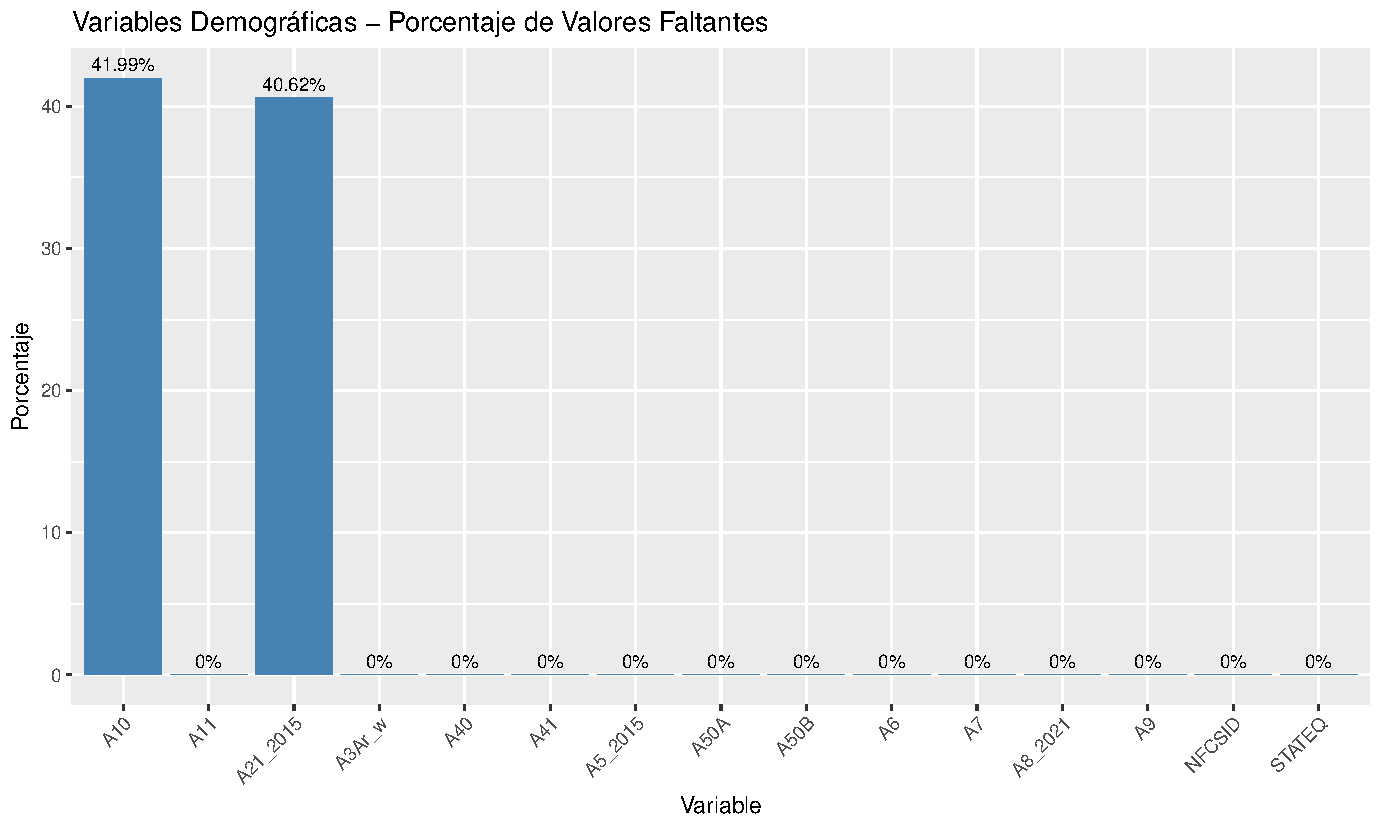
\includegraphics[width=0.8\textwidth]{images/Demographic_Features__Missing_Values.pdf} 
    \caption{Variables Demográficas: valores faltantes}
    \label{fig:demographic_features_missing_values}
\end{figure}

Comenzamos con las variables explicativas demográficas. La figure \ref{fig:demographic_features_missing_values}
recoge el porcentaje de registros que carecen de valor. Como se puede observar, solo dos 
variables explicativas tiene entradas sin definir: (1) \textbf{A10}, con un \textbf{41.99\%}
de valores faltantes y (2) \textbf{A21\_2015}, con un \textbf{40.62\%} de valores faltantes. 

Tal y como se puede consultar en la sección \ref{sec:features_description}, la 
primera de las variables corresponde con el estado laboral de la pareja y la segunda informa 
sobre estudiantes a tiempo parcial. Si bien son importantes, dado los elevados porcentajes de
datos faltantes y el elevado numero de otras variables explicativas, se opta por eliminarlas
del estudio.

La figura \ref{fig:capabilities_features_missing_values} presenta el porcentaje de valores 
faltantes para las variables explicativas correspondientes al conjunto de datos de alfabetización
financiera. En este conjunto de datos existen cuatro variables explicativas con valores faltantes:
(1) \textbf{B14}, con un \textbf{4.33\%}, (2) \textbf{C2\_2012}, con un \textbf{62.57\%}, (3) 
\textbf{C5\_2012} con un \textbf{54.04\%} y finalmente (4) \textbf{E7} con un \textbf{41.19\%}. De
nuevo, tal y como se puede comprobar en la sección \ref{sec:features_description} estas variables harían
referencia respectivamente a la inversión en acciones (B14), quién es el promotor de los planes de
pensiones (C2\_2012), si se realizan contribuciones recurrentes al plan de pensiones (C5\_2012) y
la existencia de una hipoteca (E7). En este caso, y siguiendo con el criterio introducido 
anteriormente, se eliminarán del conjunto de datos las variables con elevados porcentaje del valores faltantes y se imputará, asignando un valor sintético, la variable B14.

\begin{figure}[ht]
    \centering
    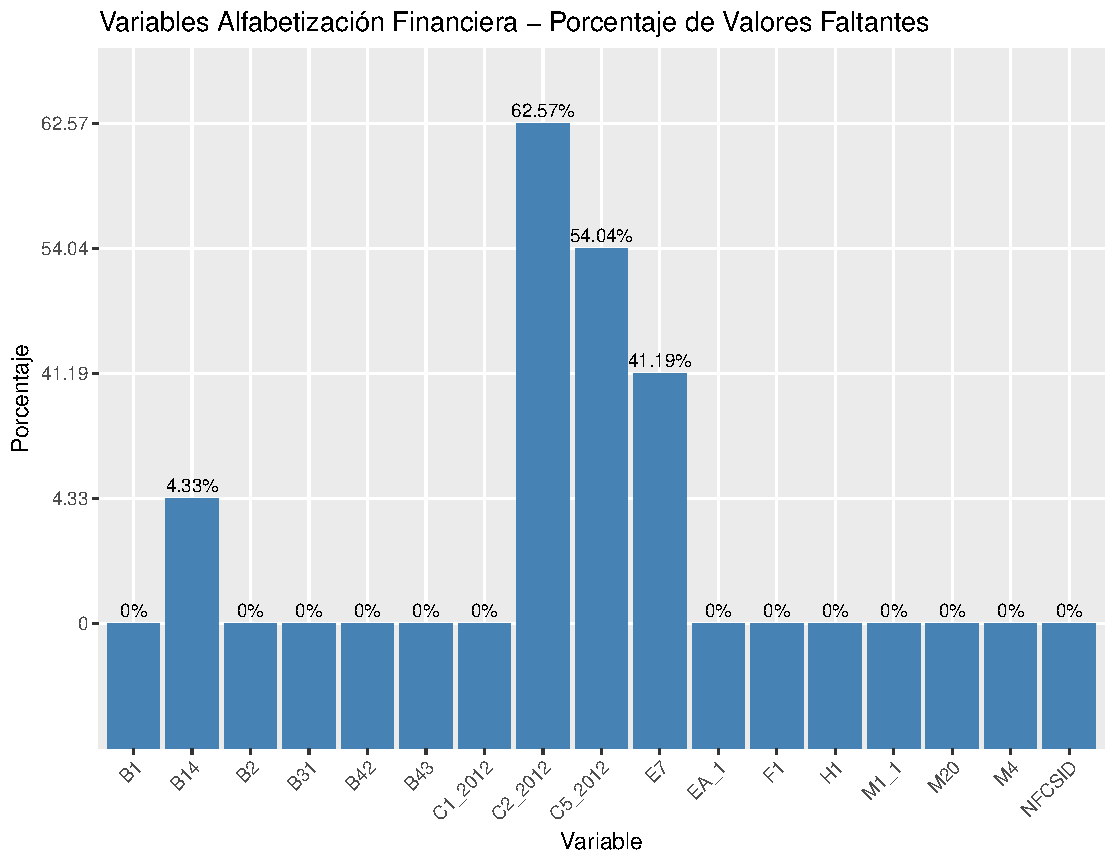
\includegraphics[width=0.8\textwidth]{images/Capabilities_Features__Missing_Values.pdf} 
    \caption{Variables Alfabetización Financiera: valores faltantes}
    \label{fig:capabilities_features_missing_values}
\end{figure}

Por último, la figura \ref{fig:stress_features_missing_values} presenta el porcentaje de valores
faltantes para las variables explicativas correspondientes al conjunto de datos de estrés
financiero. En este caso, existen 10 variables con valores faltantes: (1) \textbf{C10\_2012}, con 
un \textbf{54.04\%}, (2) \textbf{E15\_2015}, con un \textbf{69.3\%}, (3) \textbf{G35}, con un 
\textbf{76.21\%}, (4) \textbf{J6}, con un \textbf{65.6\%}, y el conjunto de variables
\textbf{F2\_1}, \textbf{F2\_2}, \textbf{F2\_3}, \textbf{F2\_4}, \textbf{F2\_5} y \textbf{F2\_6}, 
todas ellas con un porcentaje de valores faltantes de \textbf{21.09\%}. De nuevo y en pro de la 
consistencia, se descartarán del conjunto de datos aquellas variable con un elevado porcentaje
de valores faltantes. Las restantes variables, seis datos relativos a la experiencia con tarjetas 
de crédito, a pesar de contar con algo más de un 20\% de registros incompletos, serán completados
con valores sintéticos resultado de un algoritmo de imputación. 

Vale la pena resaltar que la coincidencia en los valores faltantes para variables tan relacionadas
apunta a una situación anómala en el proceso de recogida de datos, introduciendo sesgos en el estudio. 

\begin{figure}[ht]
    \centering
    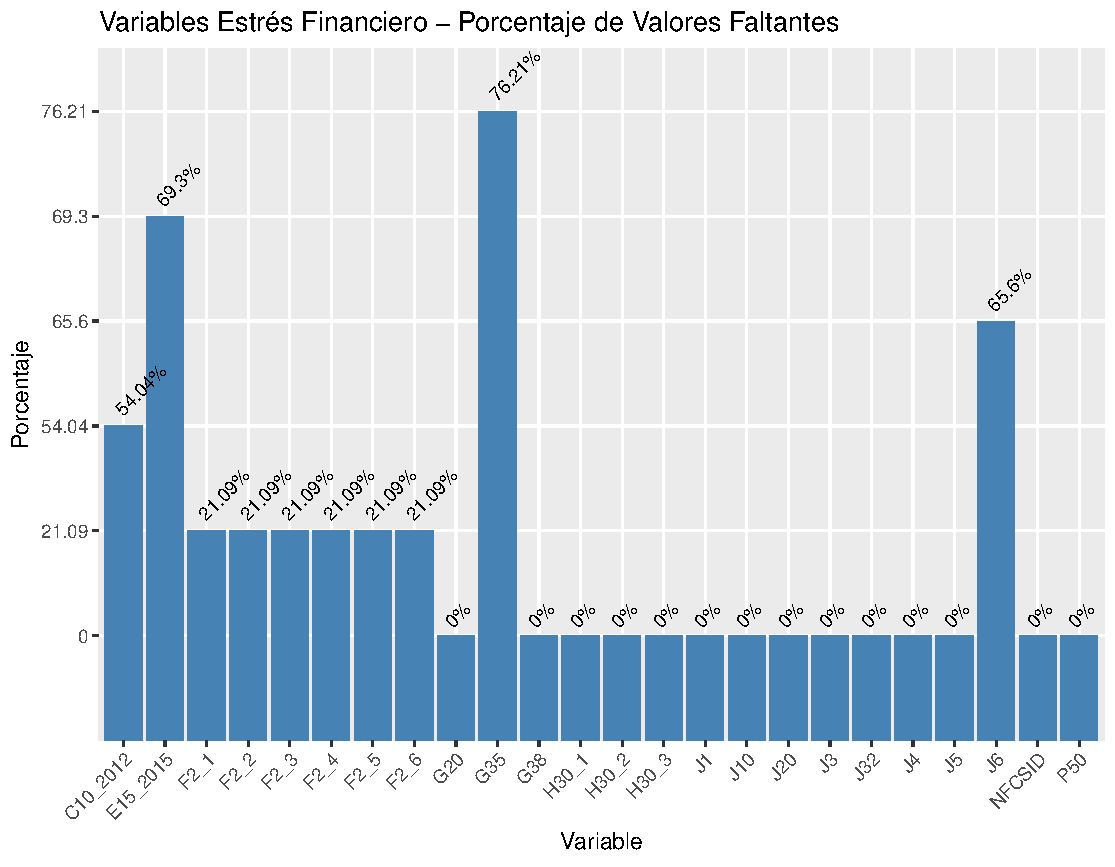
\includegraphics[width=0.8\textwidth]{images/Stress_Features__Missing_Values.pdf} 
    \caption{Variables Estrés Financiero: valores faltantes}
    \label{fig:stress_features_missing_values}
\end{figure}

El proceso de imputación de valores faltantes presenta ciertas limitaciones, derivadas de la
razón que subyace bajo la ausencia de dichos valores (ver \cite{lantz23}, pag. 572 y sucesivas). Se podría tratar de un proceso puramente aleatorio (\textbf{MCAR}), independiente 
del valor del resto de variables explicativas; simplemente, algunos valores se han perdido. 

Alternativamente, la razón que explicaría la ausencia del dato podría depender de las otras 
variables explicativas, pero no del valor ausente (\textbf{MAR}); en nuestra caso podría 
explicar los valores faltantes relativos a la experiencia con tarjetas de crédito: 
individuos sin tarjetas de crédito, difícilmente pueden tener retrasos, financiar su deuda o 
consumir todo su crédito disponible.

Finalmente los valores faltantes podrían ser una respuesta condicionada por el valor en cuestión (\textbf{MNAR}), y por lo tanto sería un resultado intencionado y no aleatorio. Un ejemplo de 
esta situación correspondería a casos en los que los individuos deciden no responder, por 
encontrar avergonzante la pregunta.

La imputación funcionará mejor en los casos en los que existe algún grado de aleatoriedad, y aunque no es posible discernir a priori la razón última que explicaría 
cada uno de los valores faltantes, merece la pena reflexionar sobre cada uno de los valores
imputados y permanecer alerta para identificar sesgos derivados del proceso.

\subsection{Datos: puesta a punto}
\label{sec:data_grooming}
Una vez revisados el conjunto de datos, se llevan a cabo operaciones de preparación y
puesta a punto. En el trabajo que nos ocupa, el proceso comenzará con la modelización
de las variables categóricas como factores, estructuras del lenguaje R, que permiten
el manejo automático de muchas de las operaciones que serán realizadas. 

Esto es necesario, ya que los datos de origen están codificados numéricamente. Sin bien, es un proceso tedioso, resulta inmediato. Con el fin de mejorar la legibilidad del código, este proceso se ha separado los ficheros independientes \textit{stress.r},
\textit{capabilities.r} y \textit{demographics.r} que forman parte del repositorio
que contiene el código del proyecto \cite{ALMO25}.

Seguidamente, se llevará a cabo el proceso de imputación o asignación de valores
sintéticos para aquellas variables explicativas seleccionadas en el aparatado anterior.
Información técnica sobre este proceso y referencias forman parte del cuadro 
explicativo incluido a continuación.
\hspace{3em}

\begin{center}
\colorbox{gray!15}{
\begin{minipage}{0.8\textwidth}
\textbf{Imputación no paramétrica}\\
  El uso de \textit{random forest}\footnote{https://academic.oup.com/bioinformatics/article/28/1/112/219101} corresponde con el estado del arte para la imputación de
  valores ausentes. Resulta especialmente recomendada para situaciones en las que se
  cuenta con variables explicativas de tipo categórico, ordinal o numérico, y es capaz
  por tanto de relaciones complejas, proporcionando además un conjunto de datos sobre
  el proceso. En R, librerías como \textit{missForest} o \textit{missRange} implementan
  el citado algoritmo que siguiendo una aproximación iterativa, modifica no solo las
  variables con valores faltantes, sino el conjunto de datos completo.
\end{minipage}}
\end{center}

A modo ilustrativo, la figura \ref{fig:Analysis_MV_B14} representa el efecto que la 
imputación tiene en la variable explicativa B14. Se puede apreciar un ligero cambio en 
la nueva distribución, consistente con el reducido porcentaje de valores faltantes.

\begin{figure}[ht]
    \centering
    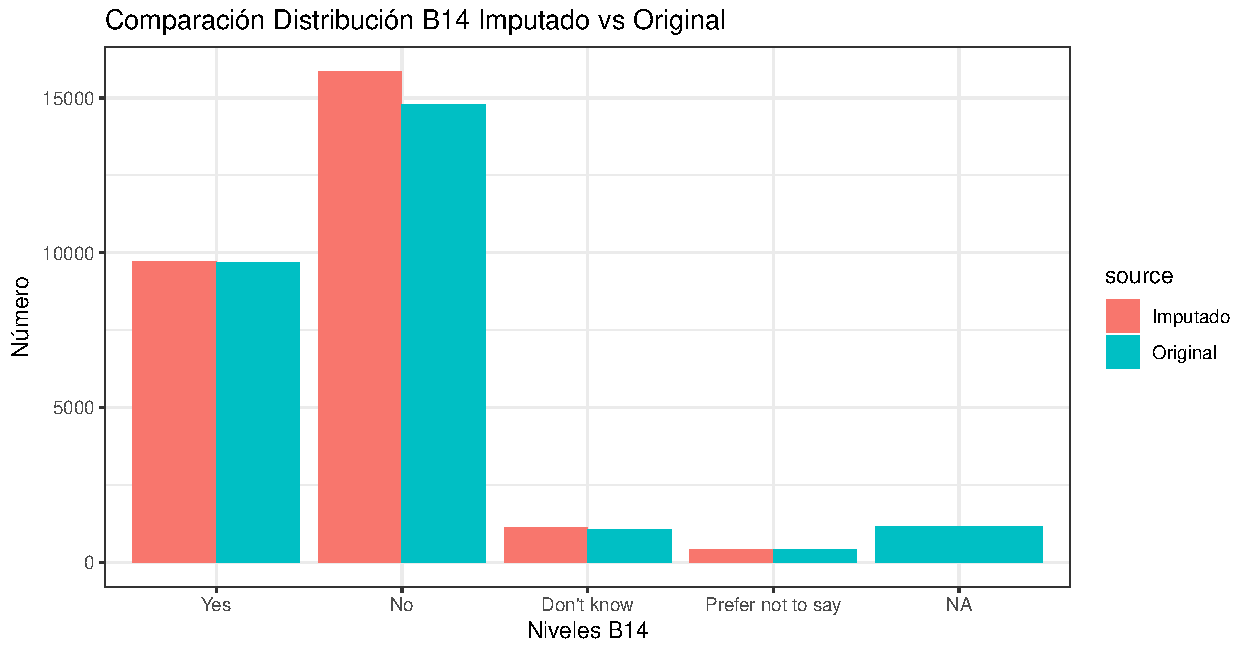
\includegraphics[width=0.8\textwidth]{images/Analysis_MV_B14.pdf} 
    \caption{Variables Alfabetización Financiera: valores faltantes}
    \label{fig:Analysis_MV_B14}
\end{figure}

En la sección \ref{sec:synthetic_analysis} se presentan las mismas figuras resumen
para las variables con valores faltantes correspondientes al conjunto de datos 
representando el estrés financiero. El resultado es muy similar para todas las 
variables ya que todas ellas presentaban un porcentaje similar de valores faltantes.
Las diferencias apreciables son debidas al las diferencias entre el resto de variables,
que hacen que el algoritmo de \textit{random forest} resulte en imputaciones ligeramente distintas.

Por último, como ya se ha mencionado, el conjunto de datos NFCS 2021 esta formado por
variables categóricas, nominales, que representan las respuestas de los participantes
al cuestionario del estudio. Si bien existe un elevado número de funciones en R que 
admiten directamente variables explicativas codificadas como factores, en el algunos
casos puede ser necesario la codificación numérica de estas. 

Anticipando esta situación,
se opta por la codificación denominada \textit{one-hot} (ver \cite{lantz23} pag. 93 y 
sucesivas). Aunque resulta inevitable si las variables son categóricas, la codificación
numérica no está exenta de problemas. Por un lado, aumenta la dimensionalidad del
problema, que en el caso de este trabajo puede ser un inconveniente añadido, ya que
el conjunto inicial de datos ya presenta una elevada dimensionalidad. Adicionalmente, 
las variables creadas presentan una elevada correlación y complica la interpretación de
los resultados.

Dicho lo cual, para cada factor, este código introduce una nueva variable binaria
por cada uno de los niveles de la categoría. Como se ha mencionado, el resultado es
la explosión dimensional del conjunto de datos y el carácter disperso de la matriz
que los representa. 

Desde el punto de vista de programación, el proceso es extremadamente sencillo, ya que R cuentan con diferentes librerías, tales como \textit{mltools} o \textit{caret}, que reducen el proceso a una única instrucción.

En la investigación que nos ocupa, y más tras el tratamiento de los valores faltantes, los
conjuntos de datos no son especialmente grandes, por lo que el impacto de la codificación
\textit{one-hot} no será importante; en particular el conjunto de datos demográficos pasa
de 13 a 131 dimensiones, el conjunto de datos de alfabetización financiera pasa de 14 a 72
dimensiones y el conjunto de datos de estrés financiero para de 20 a 92 dimensiones.

\subsection{Métodos y parametrización}
\label{sec:sub:clustering}
Una vez preparados los conjuntos de datos, el primer paso consiste en la definición de
una taxonomía que permita clasificar los individuos de acuerdo con su estrés financiero.
Como no se cuenta con información previa, se trata de un proceso de aprendizaje no supervisado,
que requiere un análisis detallado de la información disponible. En este punto, la exploración
de los datos, proporciona al investigador indicios sobre los que establecer hipótesis que
se contrastarán durante la investigación. En este caso, nuestro objetivo es determinar el
número de categorías que parametriza los algoritmos no supervisados y la evidencia que 
proporcionan las distintas variables explicativas, para seleccionar las más adecuadas en el
proceso de clasificación supervisado.

Técnicas como el Análisis de Componentes Principales (\textit{Principal Component
Analysis} (PCA)) y la aproximación para variables categóricas que permite la denominada
Análisis de Correspondencia Múltiple (\textit{Multiple Correspondence  Analysis}
(MCA))\cite{Husson20} permiten explorar, en un dominio de elevada dimensionalidad, la 
inercia, varianza del conjunto de datos explicada, de cada variable explicativa y 
obtener una idea aproximada de las categorías presentes. Esto también permite valorar el 
carácter discriminante de las distintas variables.

\begin{figure}[ht]
    \centering
    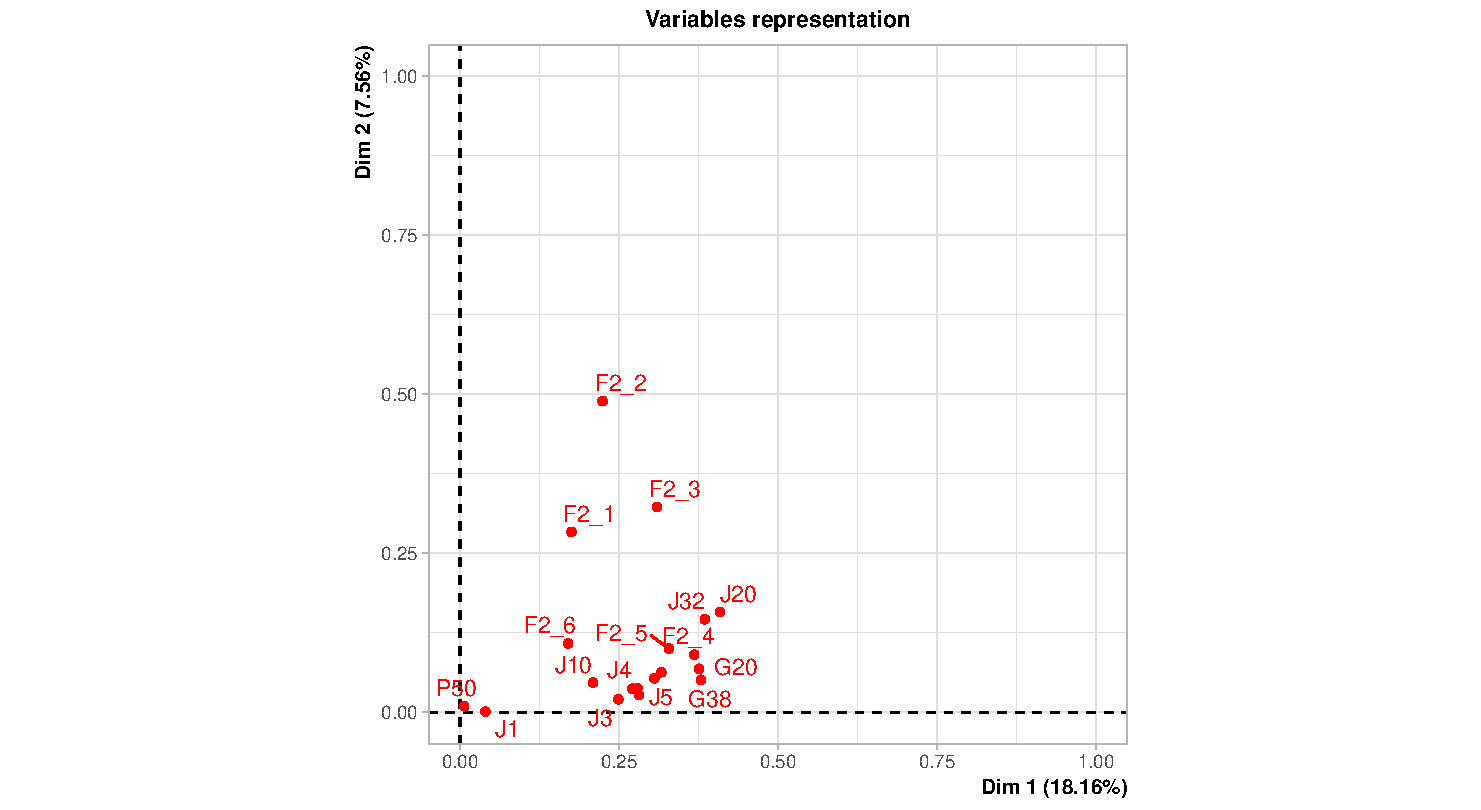
\includegraphics[width=0.8\textwidth]{images/mca_stress_features_inertia.pdf} 
    \caption{Análisis MCA: inercia de las variables explicativas}
    \label{fig:mca_stress_features_inertia}
\end{figure}

El conjunto de datos correspondiente al estrés financiero esta formado por 20 variables 
explicativas y una muestra de algo más de 27000 individuos. Esta elevada dimensionalidad
exige simplificar el proceso, reduciendo el número de muestras hasta el punto en el que 
el proceso computacional es ejecutado en un tiempo razonable y los resultados gráficos, de
importancia significativa en estas técnicas, puedan ser analizadas satisfactoriamente. En 
nuestro caso, el estudio se realiza con un 2\%, 542 individuos, de la muestra completa y 
excluyendo la variable que identifica de manera única el registro correspondiente. 
Adicionalmente se parametriza el análisis MCA para colapsar grupos con menos del 10\% de
individuos. 

Tal y como se observa en la figura \ref{fig:mca_stress_features_inertia}, el conjunto de
variables explicativas del estrés financiero, proyectadas en dos dimensiones, explican
aproximadamente el 26\% de la varianza del conjunto de datos, con contribuciones 
principalmente de variables como F2\_2, F2\_1, F2\_3 (tarjetas de crédito), J20 (capacidad
para afrontar imprevistos) o J32 (rating crediticio).

\begin{figure}[ht]
    \centering
    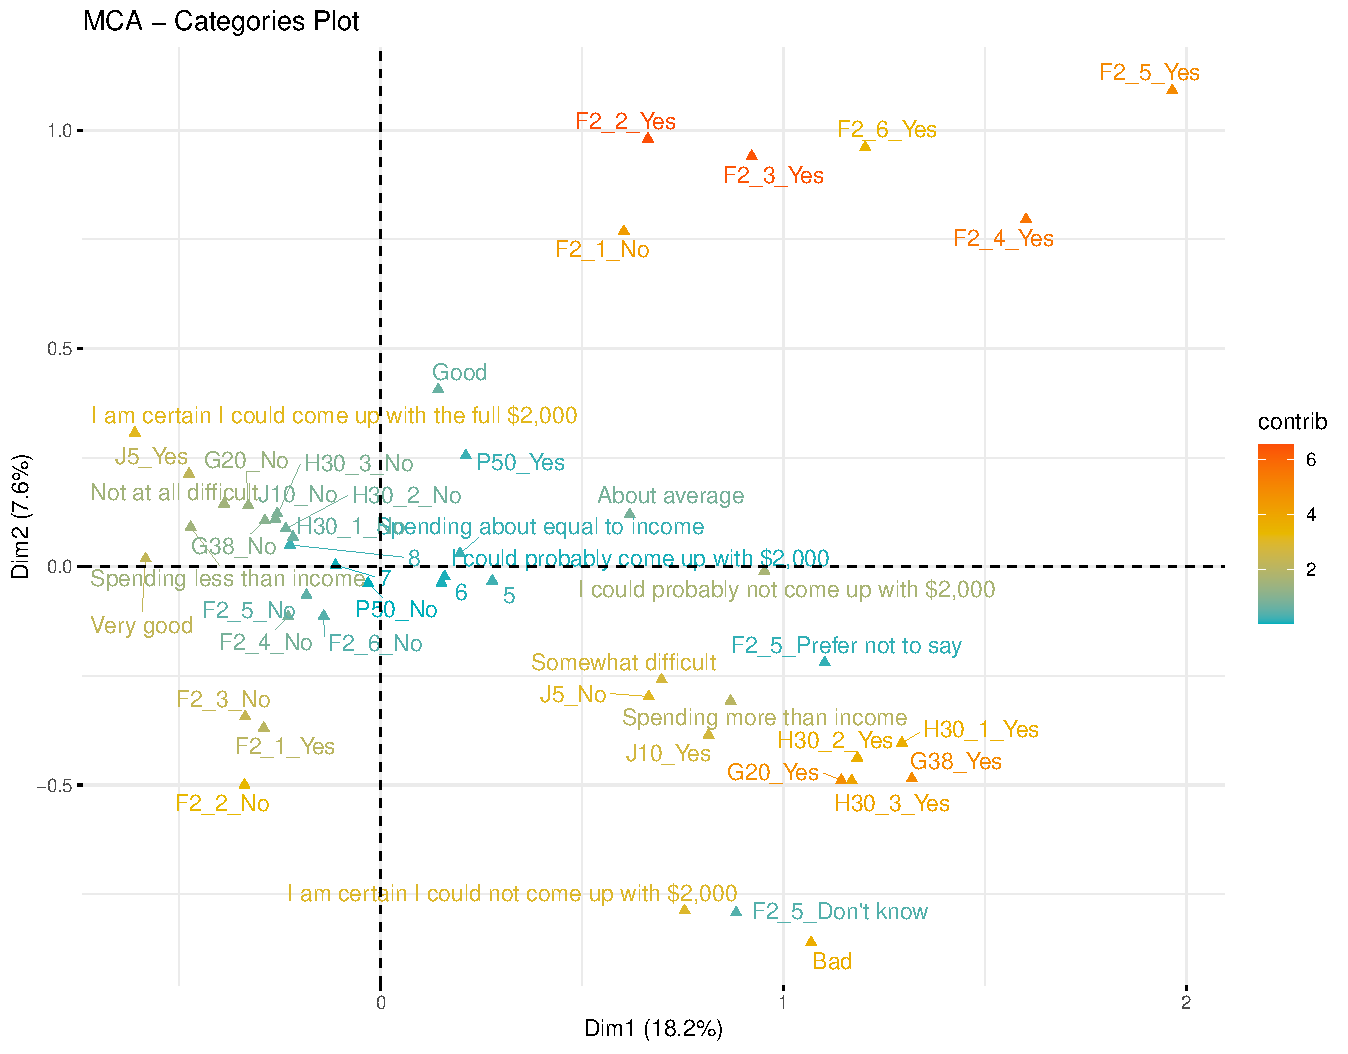
\includegraphics[width=0.8\textwidth]{images/mca_stress_categories.pdf} 
    \caption{Análisis MCA - Categorías}
    \label{fig:mca_stress_categories}
\end{figure}

En la figura \ref{fig:mca_stress_categories} se recogen las contribuciones a nivel 
de categorías, combinación variable explicativa y valor. Esta combinación resultará
de utilidad una vez se evalúe los grupos de individuos clasificados de manera no 
supervisada. A continuación se ha realizado el análisis de las variables explicativas 
que según hemos visto en el párrafo anterior, permiten explicar una elevada proporción
de la varianza. La figura \ref{fig:mca_stress_fX_Y_ellipses} recoge los resultados para
el conjunto de variables explicativas relativas a el uso de tarjetas de crédito. Tal
y como muestran las figuras, los grupos son claros y deberían verse reflejados posteriormente.

\begin{figure}[ht]
    \centering
    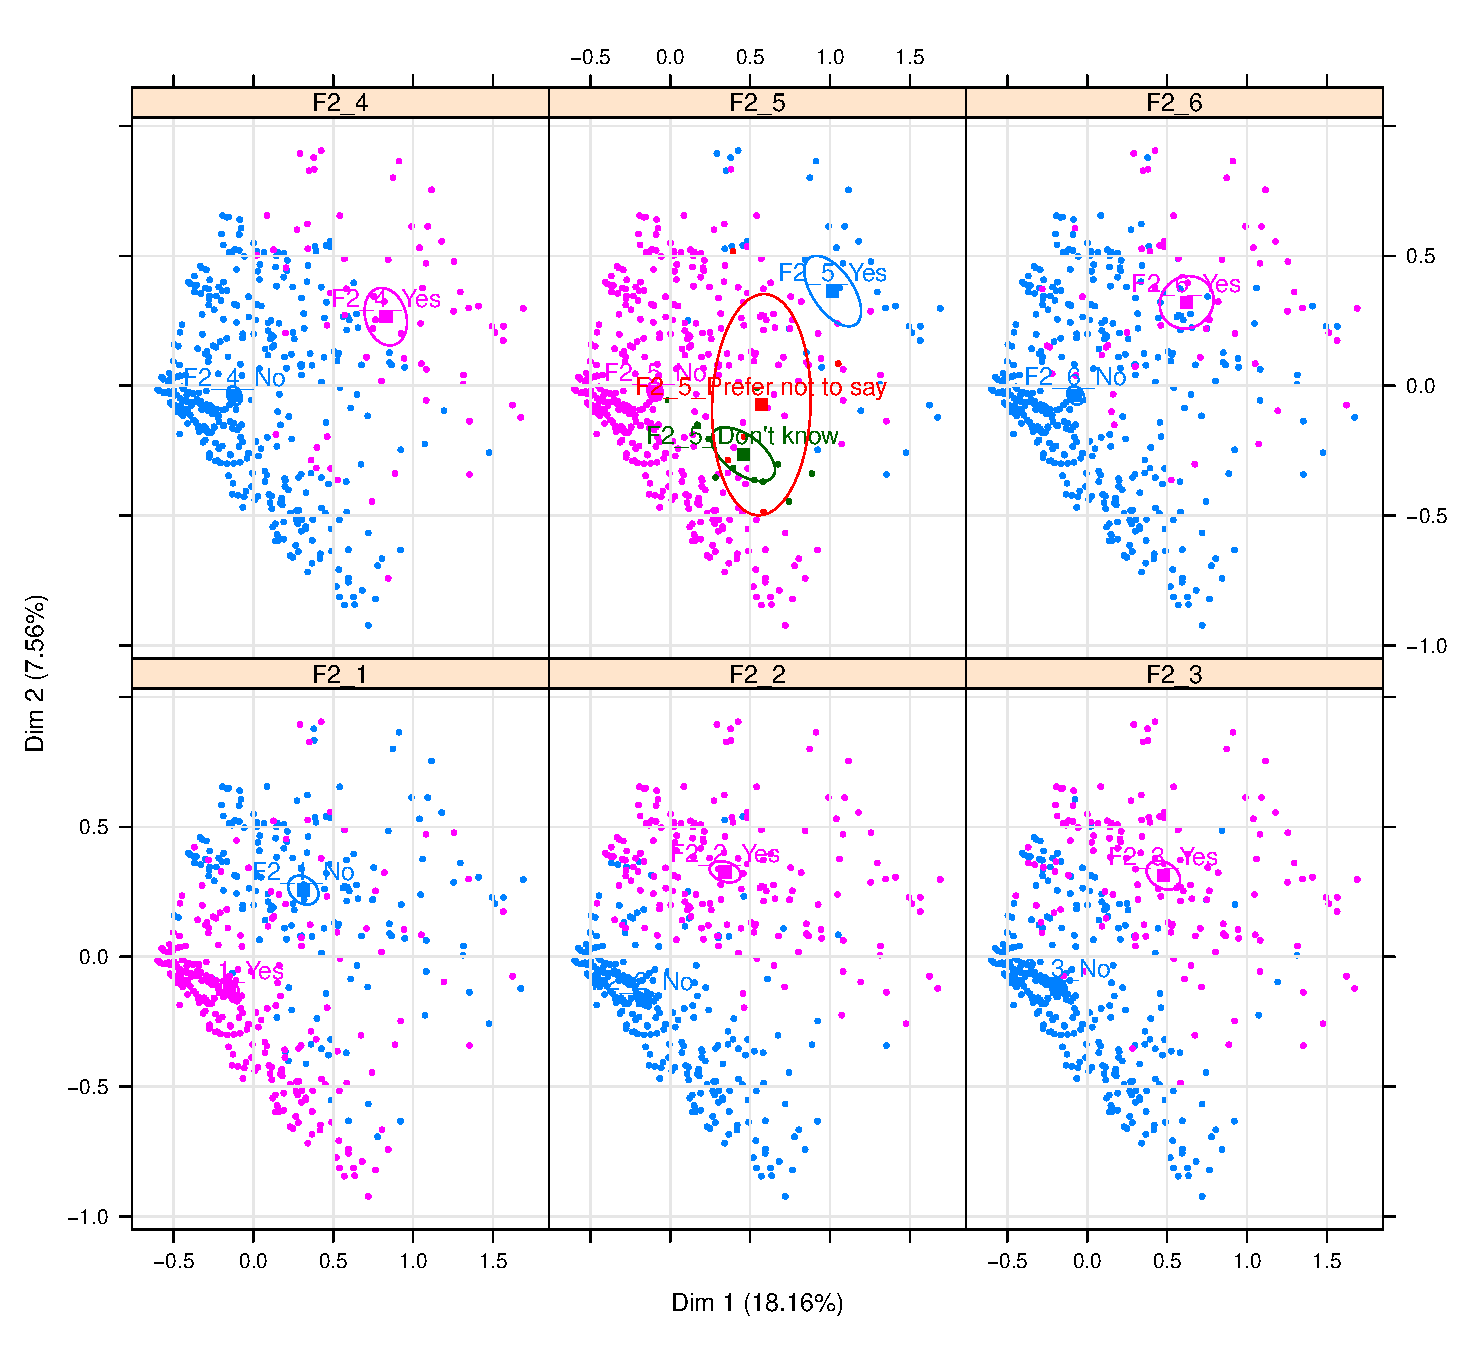
\includegraphics[width=0.8\textwidth]{images/mca_stress_fX_Y_ellipses.pdf} 
    \caption{Análisis MCA - F2\_2, F2\_1, F2\_3, F2\_4, F2\_5 \&, F2\_6}
    \label{fig:mca_stress_fX_Y_ellipses}
\end{figure}

De igual forma, la figura \ref{fig:mca_stress_j20_j32_ellipses} presenta el análisis para las
variables J20 y J30. En estos casos, las variables categóricas presentan algunos niveles 
adicionales, produciendo una representación menos concluyente. Aun a si, es posible identificar 
con claridad algunas agrupaciones, que sin duda también resultarán de utilidad mas adelante.

\begin{figure}[ht]
    \centering
    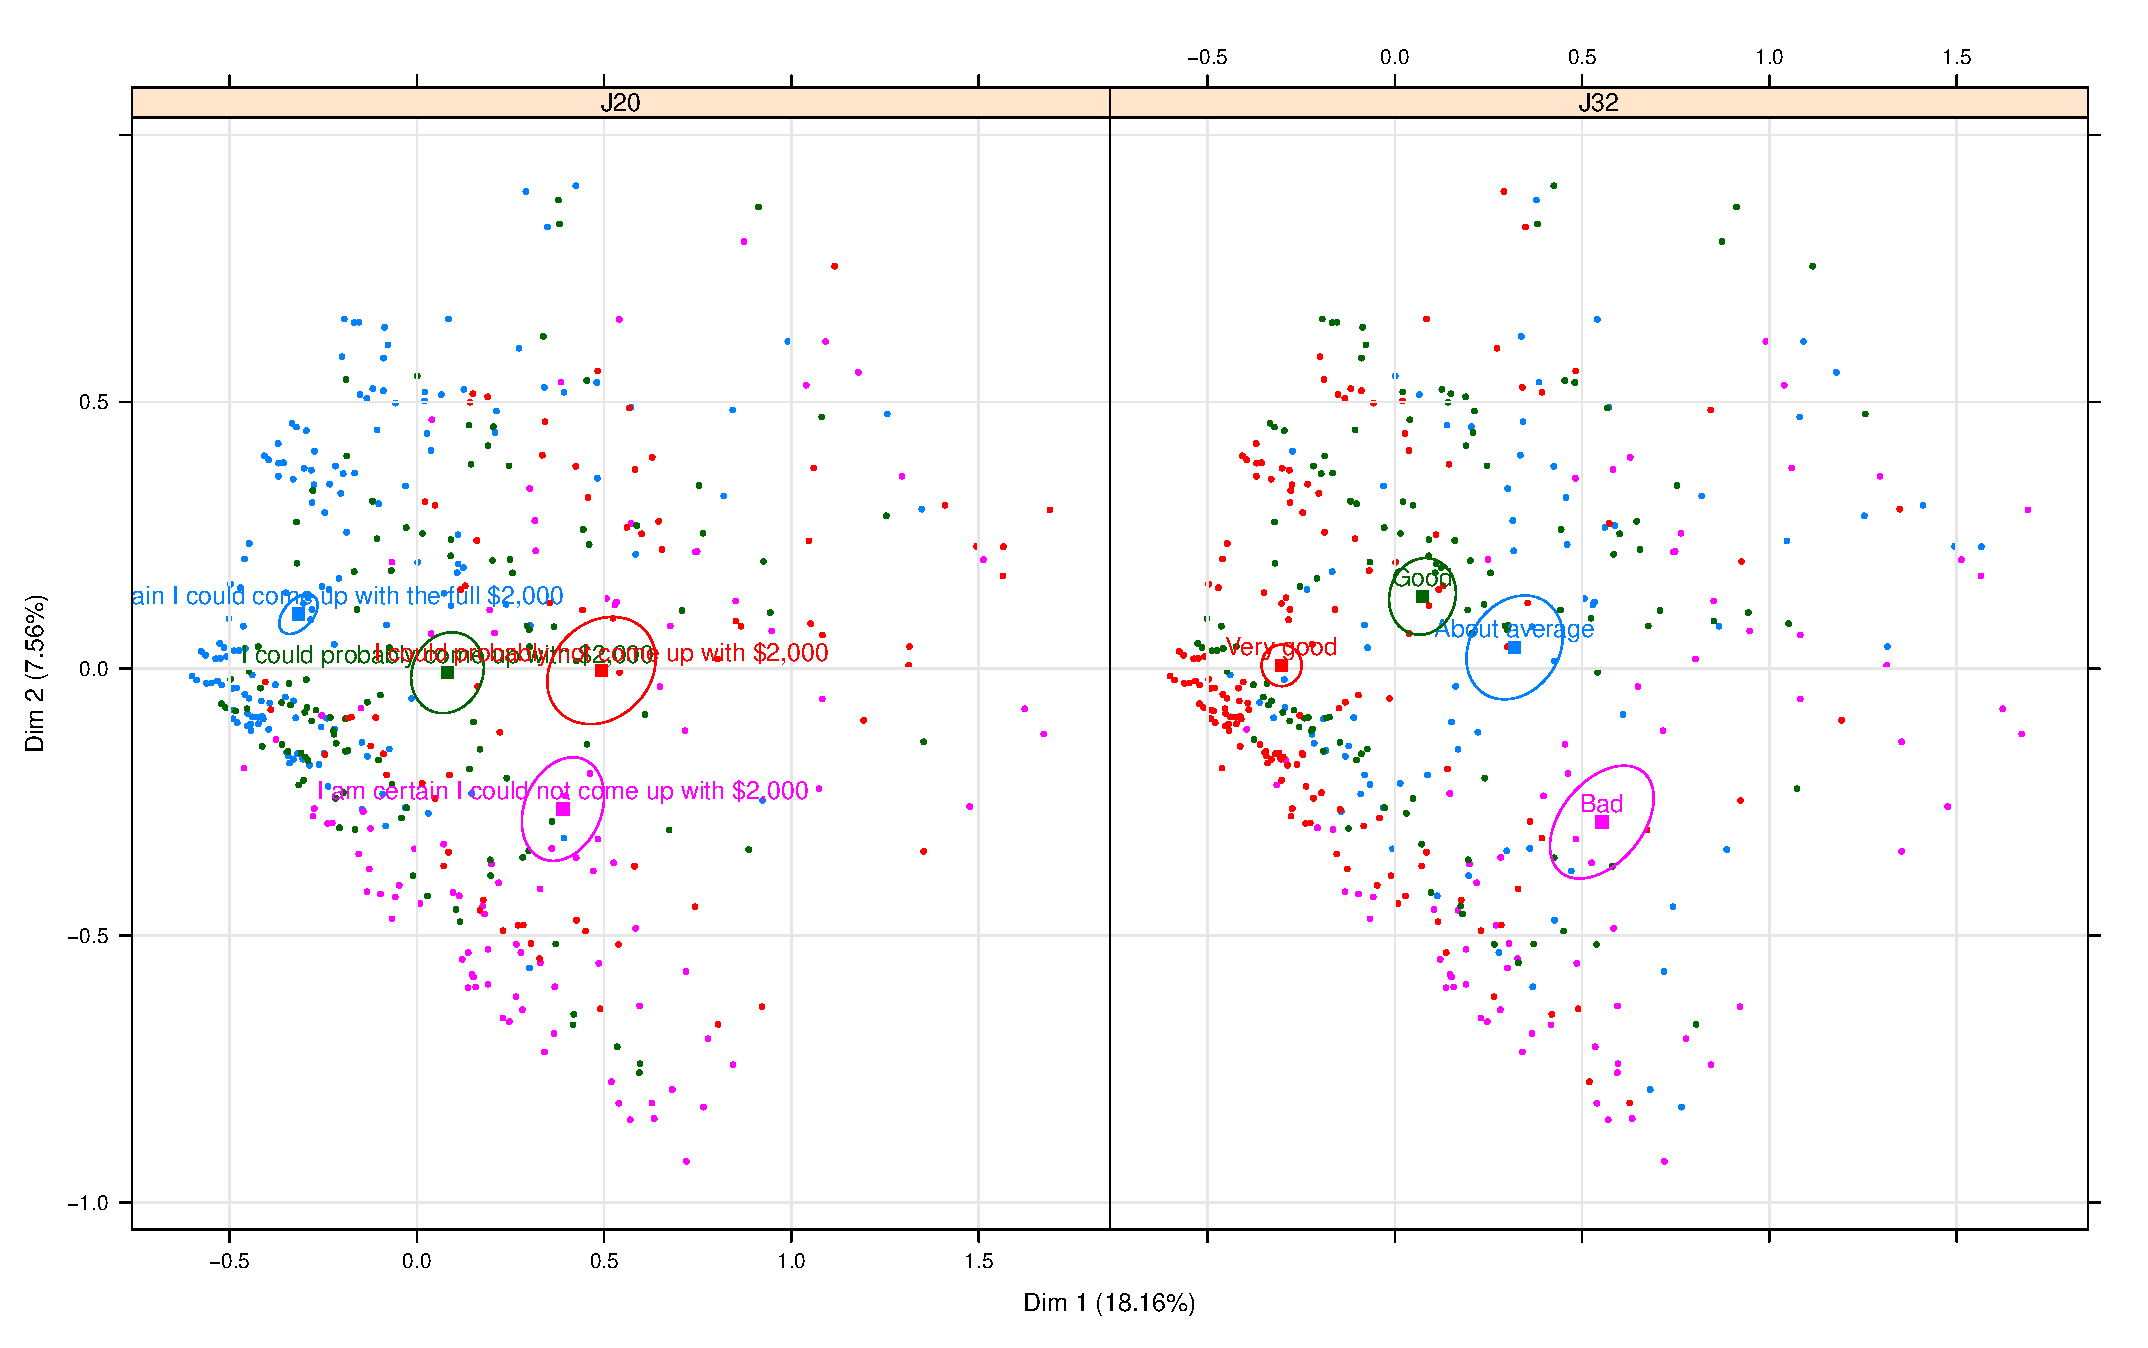
\includegraphics[width=0.8\textwidth]{images/mca_stress_j20_j32_ellipses.pdf} 
    \caption{Análisis MCA - J20 \& J32}
    \label{fig:mca_stress_j20_j32_ellipses}
\end{figure}

Una vez completado el análisis exploratorio, el siguiente paso será lleva a cabo 
clasificación no supervisada, para lo que se empleará el algoritmo de k medias
\cite{Hastie23}. En este caso, una vez mas, debido a que nuestro conjunto
de datos es de carácter categórico nominal, se utilizará la variantes denominada
k modas. En cualquier caso, el algoritmo requiere un parámetro principal: el número
de grupos a definir. 

Tal y como hemos visto durante el análisis exploratorio, un 
número entre 3 y 5 puede ser razonable. Desde un punto de vista de la investigación, 
parece sensato reducir el número al máximo para facilitar el análisis. Es más, teniendo
en cuenta que el proceso es no supervisado, parece recomendable una primera aproximación 
de grano grueso. En cualquier caso, existen técnicas para obtener una recomendación en
base a un análisis cualitativo, que se fundamentan en una métrica de coherencia entre
los grupos identificados. 

En esta investigación utilizaremos las técnicas \textit{Elbow Method} y \textit{Silhouette Method},
ambas basadas la denominada distancia inter grupos, que hacen uso de una métrica adaptada 
para variables categóricas. Realizando una comparativa para grupos de entre 2 y 10 categorías, 
los resultados para ambas técnicas pueden comprobarse en la figura \ref{fig:k-modes-hyperparameters}. De acuerdo con el \textit{Elbow Method} no existe un valor claro,
mientras que siguiendo el \textit{Silhouette Method}, el valor recomendado sería de 3 grupos.
En cualquier caso, merece la pena recordad que estos métodos son recomendaciones que 
orientan en última instancia al investigador. Sumadas al criterio, el contexto y la necesidad
posterior, podrán elegirse un número distinto o lo que es más probable, combinar análisis
con distintos grupos según el caso.

A continuación se realizará un proceso de clasificación del conjunto de datos que modelizan
el estrés financiero. De acuerdo al análisis exploratorio y la necesidad de mantener un
valor reducido de categorías para facilitar el análisis posterior, clasificaremos el 
conjunto de datos en tres grupos. En términos de programación, esto es extremadamente
sencillo, limitándose a una llamada en R.

Aunque los resultados se analizaran desde el punto de vista económico en la siguiente sección,
en este apartado se presentan algunos detalles del los resultados. El algoritmo clasifica
todas las instancias, organizándolas, según el parámetro proporcionado, en tres grupos:
(1) nivel 1, 14271 individuos, (2) nivel 2, 8926 individuos y (3) nivel 3, con 3921 
individuos. Revisando los criterios introducidos, se observan cuatro variables explicativas
sin capacidad discriminante, esto es, presentan un mismo valor para los tres grupos. 

Una vez obtenidas las clasificaciones o taxonomías anteriores, y tras etiquetar los conjuntos
adecuadamente, se desarrollarán, utilizando un aprendizaje supervisado, clasificadores que 
permitan partiendo de los datos demográficos o de alfabetización financiera determinar el 
nivel de estrés financiero, ya sea para recomendar medidas de alfabetización financiera 
paliativas o de prevención.
\begin{center}    
\begin{figure}[ht]
    \centering
    \begin{subfigure}[t]{0.45\linewidth}
        \centering
        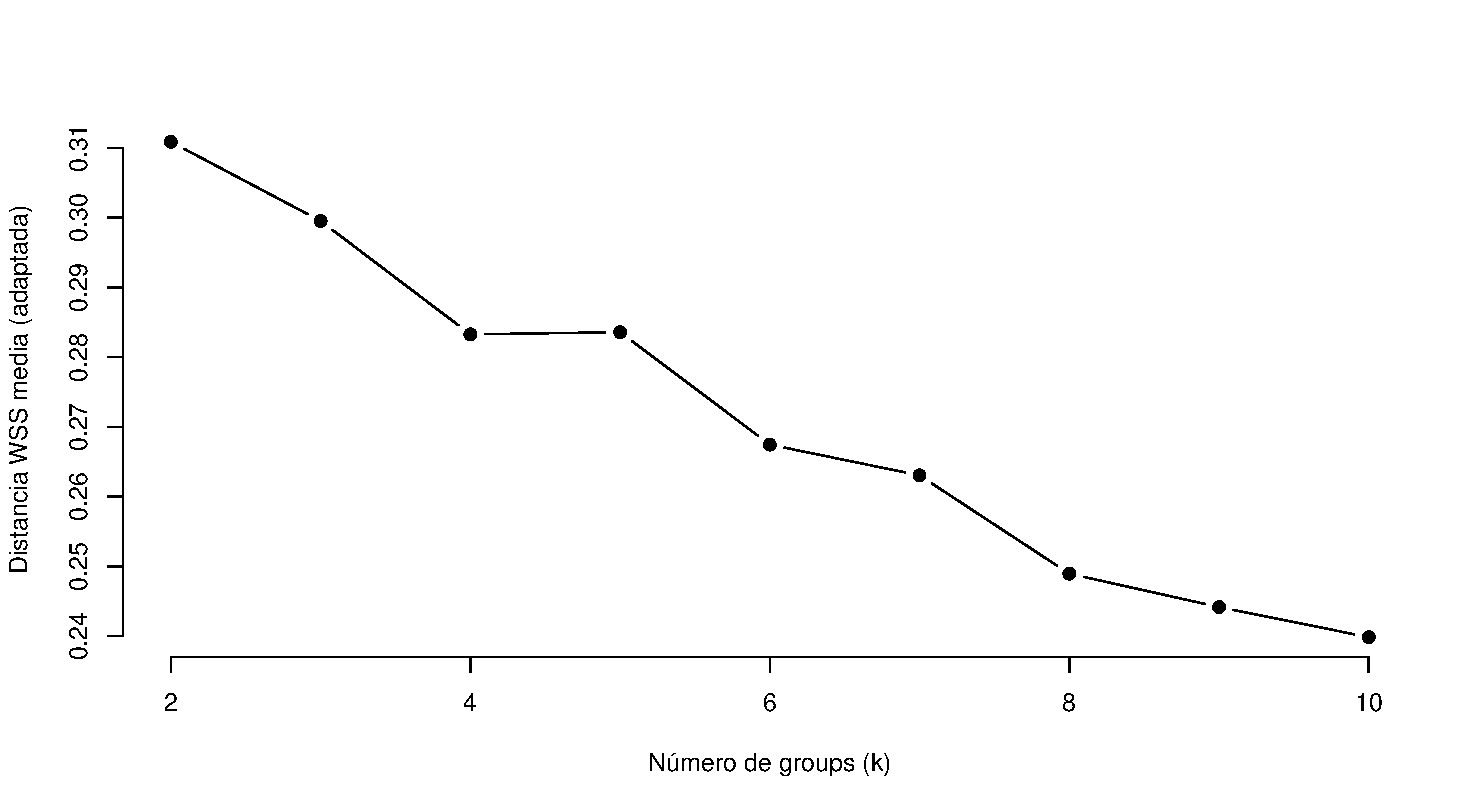
\includegraphics[width=\linewidth]{images/clustering_wss_analysis.pdf}
        \caption{Elbow Method}
        \label{fig:clustering_wss_analysis}
    \end{subfigure}
    \hfill 
    \begin{subfigure}[t]{0.45\linewidth}
        \centering
        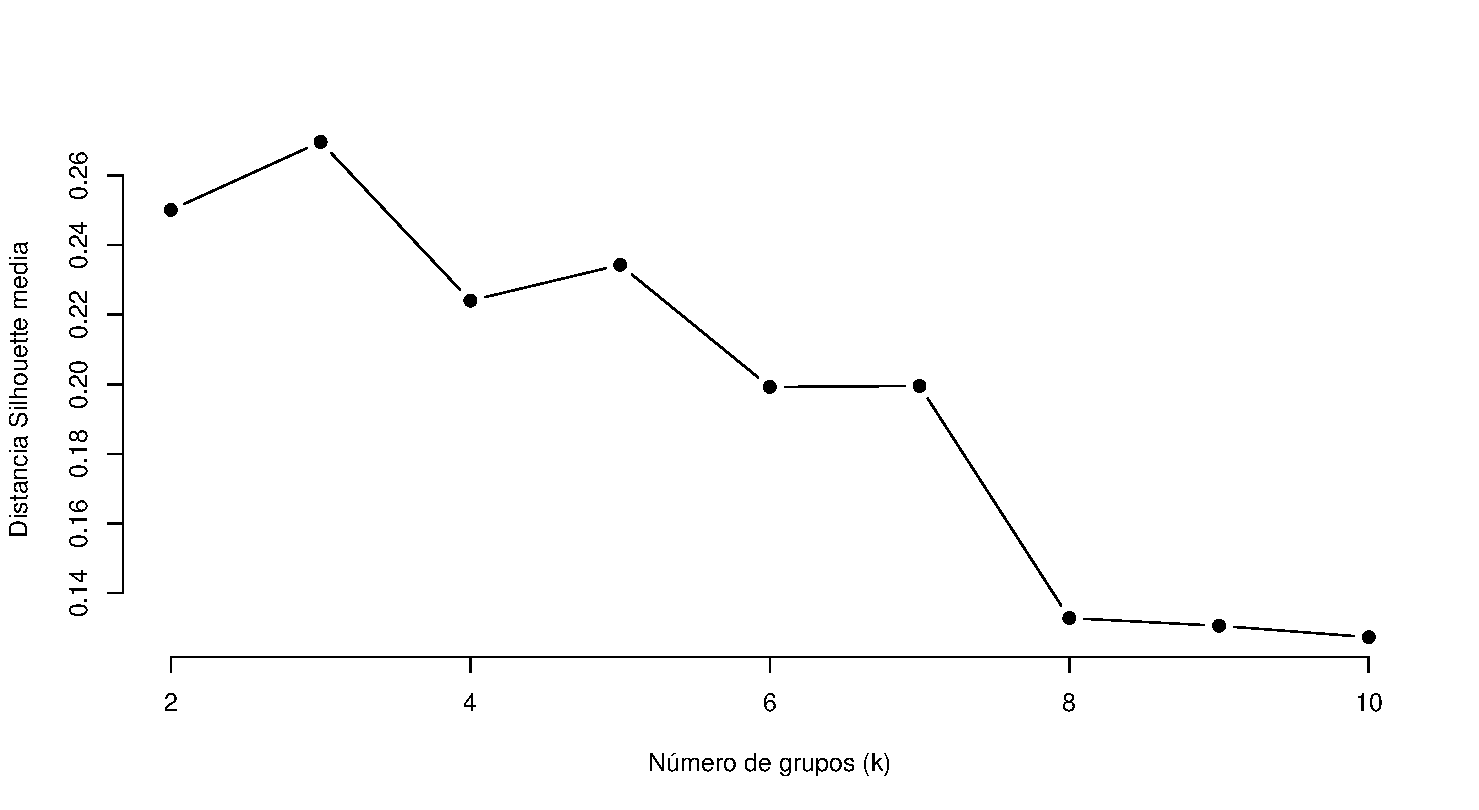
\includegraphics[width=\linewidth]{images/clustering_silhouette_analysis.pdf}
        \caption{Silhouette Method}
        \label{fig:clustering_silhouette_analysis}
    \end{subfigure}
    \caption{Parametrización del algoritmo K Modas}
    \label{fig:k-modes-hyperparameters}
    \end{figure}
\end{center}

Una pregunta que surge de manera inmediata es cómo el criterio seguido para agrupar los datos
correspondientes al estrés financiero permiten clasificar el conjunto de datos completo. Para
evaluar esto, se vuelve a realizar el análisis de correspondencia múltiple, ahora con el
conjunto de datos completo, aumentado con una nueva variable explicativa que representa 
los grupos de estrés financiero obtenidos con el algoritmo de k modas. Los resultados 
se recogen en la figura \ref{fig:clustering_nfcs_stress}. Tal y como se puede apreciar, si bien
existe una elevada concentración de valores, los grupos definidos resultan apreciables. Una
vez que se evalúen los algoritmos de clasificación supervisados se podrá determinar la 
precisión alcanzada.

\begin{figure}[ht]
    \centering
    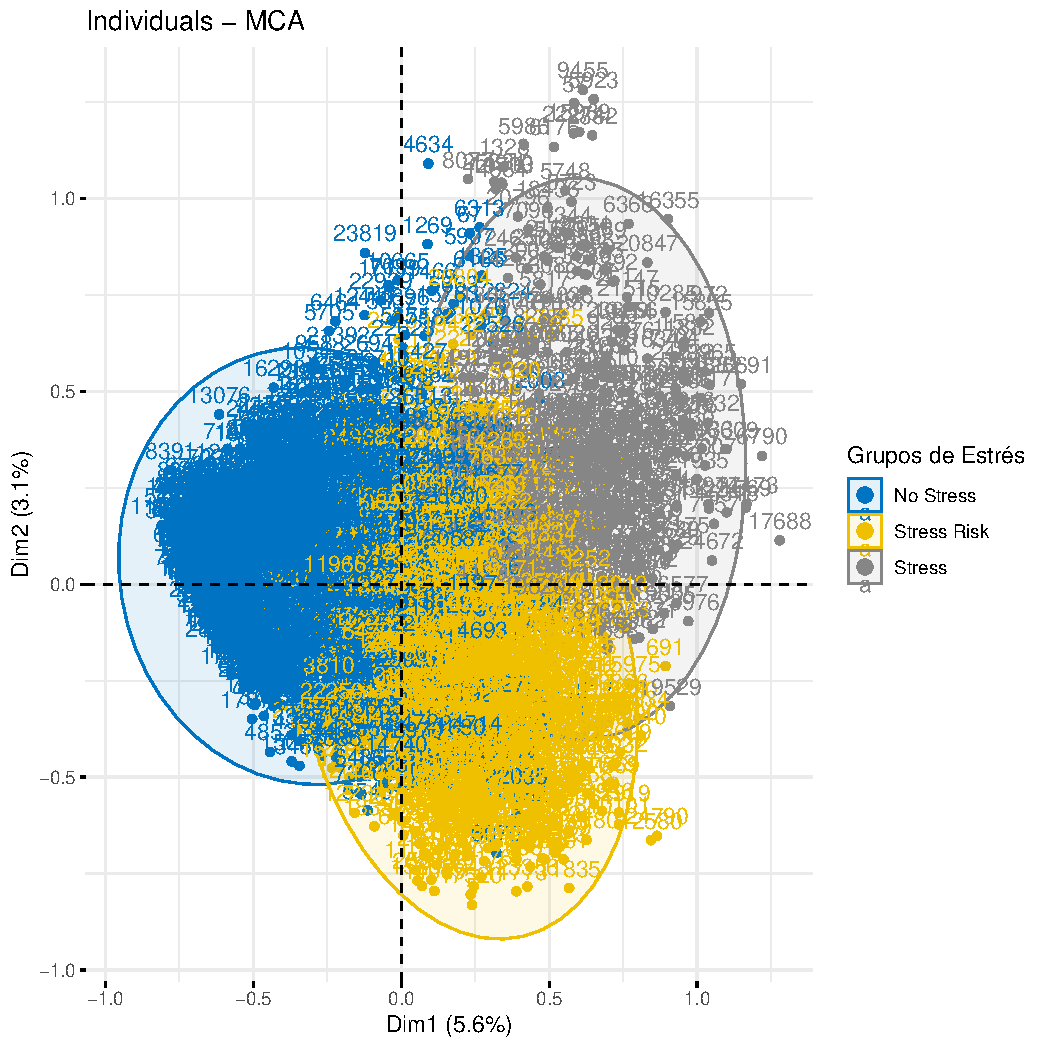
\includegraphics[width=0.9\textwidth]{images/clustering_nfcs_stress.pdf} 
    \caption{Clasificación de NFCS usando Grupos de Estrés}
    \label{fig:clustering_nfcs_stress}
\end{figure}

Partiendo de los datos catalogados bajo la taxonomía introducida con los niveles de 
estrés financiero, en el siguiente paso se lleva a cabo la evaluación de los 
clasificadores automáticos. Las distintas técnicas existentes responde de manera 
diferente, por lo que el proceso de evaluación permitirá comprobar la bondad de 
cada uno de ellos. Las técnicas que se evaluarán a continuación son: (1) 
\textit{random forest}, (2) máquinas de vector soporte (\textit{Support 
Vector Machine} (SVM)), y (3) clasificadores bayesianos (Naive Bayes).

El proceso es similar en todos ellos, variando únicamente algunos de los parametros 
requeridos. La secuencia que se sigue es la siguiente:
\begin{description}
    \item[Datos] El conjunto de datos es el resultado de unir los 
    datos correspondientes a la información demográfica y la información sobre 
    alfabetización financiera, junto con el grupo de estrés, síntesis de la información
    sobre estrés financiera procesa durante el primer paso. Tras esto, se generan las
    muestras de entrenamiento y test, que permitirán el desarrollo del clasificador y
    su validación.
    \item[Entrenamiento] Con la información preparada en el paso anterior
    se realiza el entrenamiento, limitando la muestra de los datos y ajustando los parámetros
    que sean necesarios. El clasificador deberá calcular el grupo de estés haciendo uso de 
    las 25 variables explicativas\footnote{La lista de variables es la siguiente: STATEQ, A50A,
    A3Ar\_w, A50B, A5\_2015, A6, A7, A11, A8\_2021, A9, A40, A41, B1, B2, B31, B42, B43, C1\_2012,
    B14, EA\_1, F1, H1, M1\_1, M4 y M20. La descripción de todas ellas se puede consultar en la sección \ref{sec:features_description}.} que forman el conjunto de datos, tras el proceso de
    preparación. 
    \item[Validación] Completada la fase de entrenamiento, el clasificador se 
    valida evaluando los resultados con la muestra de datos de prueba. El resultado será una
    matriz confusión que
\end{description}
Los resultados se muestran en la tabla \ref{tab:clasifiers_comparative}, que incluye la
precisión del clasificador, más la precisión que se obtendría respondiendo siempre con la
clase más frecuente, así como el P-value que contrasta si hay diferencia entre ellos. 
Como se puede comprobar los clasificadores sobre bastante pobres. Como caso extremo, el
clasificador de máquina de vectores soporte no cuenta con suficiente evidencia (P-Value 
elevado) como para descartar el que no hay diferencia entre responder siempre con la 
clase más frecuente y el clasificador.

Una vez evaluados los diferentes clasificadores, el siguiente paso consistiría en la mejora
de los modelos, comenzando con el ajuste de los parámetros. Este ajuste se puede realizar
mediante la comparación de los modelos resultantes de la modificación controlada de los 
parámetros o de forma más fundamentales, modificando la selección de variables explicativas.
Tras estos ajustes, se pueden abordar cambios más drásticos, modificando la muestra o incluso
los fundamentos del experimento.

\begin{table}[ht]
\centering
\begin{tabular}{lc}
\toprule
\textbf{} & \textbf{Value} \\
\midrule
\textbf{Random Forest} & \\
\hspace{1em} Accuracy & 0.649 \\
\hspace{1em} Pre. Clase Frec. (NIR) &  0.5244\\
\hspace{1em} P-Value [Acc $>$ NIR] &  $<$ 2.2e-16\\
\textbf{Support Vector Machine} & \\
\hspace{1em} Accuracy &  0.5249 \\
\hspace{1em} Pre. Clase Frec. (NIR) & 0.5244\\
\hspace{1em} P-Value [Acc $>$ NIR] &  0.4414\\
\textbf{Naive Bayes} & \\
\hspace{1em} Accuracy &  0.6451 \\
\hspace{1em} Pre. Clase Frec. (NIR) &  0.5244\\
\hspace{1em} P-Value [Acc $>$ NIR] &  $<$ 2.2e-16\\
\bottomrule
\end{tabular}
\caption{Clasificadores: Comparativa}
\label{tab:clasifiers_comparative}
\end{table}

Llegado a este punto, este apartado completa la exploración y análisis de las técnicas empleadas, 
para pasar a abordar el análisis económico de la taxonomía del estrés financiero. Aun siendo 
conscientes de las limitaciones de las técnicas desarrolladas, este ejercicio interpretativo
persigue ilustrar los resultados que podrían extraerse de la aplicación de técnicas de aprendizaje
automático (\textit{machine learning}). 

\section{Resultados: análisis y evaluación}
\label{sec:results_analysis}
Como se mencionó en la introducción, el objeto que persigue este estudio es la aplicación
de técnicas de aprendizaje automático en un dominio donde las técnicas econométricas 
presentan limitaciones. Las principales características de este dominio son: (1) un elevado
número de variables explicativas de carácter categórico, lo que se traduce en una elevada 
dimensionalidad y (2) la disponibilidad de una muestra grande, con varios miles de registros, 
que hace viable la aplicación de técnicas intensivas en consumo de datos.

En particular, la información de alfabetización financiera es el punto de partida para, en primer
lugar introducir el concepto de estrés financiero, educido de forma no supervisada de un subconjunto
de datos de la colección principal. Una vez etiquetados los registros del conjunto de datos, se 
han desarrollado clasificadores, que partiendo de datos demográficos o de alfabetización financiera
\footnote{Excluidas aquellas variables representadas sintéticamente por el grupo de estrés financiero
asignado.} permitan catalogar el riesgo financiero del individuo, pudiendo anticipar medidas de 
prevención, idealmente, o de mitigación en el peor caso.

En esta sección de análisis se precederá a la interpretación que, del conjunto de datos completo, 
permite hacer la asignación de los grupos de riesgo. Otros aspectos, sin duda interesantes, 
requerirían la expansión del ámbito de investigación, por lo que quedan fuera del alcance de
este estudio.
\subsection{Taxonomía del estrés financiero}
\label{sec:financial_stress_taxonomy}

El análisis realizado categoriza los individuos del conjunto de datos en tres grupos:
(1) No estrés financiero, (2) Riesgo de estrés financiero y (3) Estrés financiero. Esta
taxonomía se establece en función de los valores de las variables explicativas manejadas
(ver \ref{sec:features_description}) de acuerdo a los valores recogidos en la tabla 
\ref{tab:stress_taxonomy}

\begin{table}
\centering
\begin{tabular}{ |p{1cm}||p{3.2cm}|p{3.2cm}|p{3.2cm}|  }
\hline
  & \textbf{Grupo 1}  &  \textbf{Grupo 2} & \textbf{Grupo 3}\\
 \hline
  \hline
 \textbf{J1} & \textit{Satisfied} (8) & \textit{Satisfied} (1) & \textit{Satisfied} (1) \\
 \hline
 \textbf{J3} & \textit{Spending less than income} & \textit{Spending about equal to income} & \textit{Spending more than income} \\
 \hline
 \textbf{J4} & \textit{Not at all difficult} & \textit{Somewhat difficult} & \textit{Somewhat difficult} \\
 \hline
 \textbf{J5} & \textit{Yes} & \textit{No} & \textit{No}\\
 \hline
 \textbf{J10} & \textit{No} & \textit{No} & \textit{Yes} \\
 \hline
 \textbf{J20} & \textit{I am certain I could come up with the full \$2,000}& \textit{I could probably come up with \$2,000}
 & \textit{I am certain I could not come up with \$2,000}\\
 \hline
 \textbf{J32} & \textit{Very good} & \textit{Good}& \textit{About average} \\
 \hline
 \textbf{F2\_1} & \textit{Yes} & \textit{Yes} & \textit{No} \\
 \hline
 \textbf{F2\_2} & \textit{No} & \textit{No} & \textit{Yes}\\
 \hline
 \textbf{F2\_3} & \textit{No} & \textit{No} & \textit{Yes}\\
 \hline
 \textbf{F2\_4} & \textit{No} & \textit{No} & \textit{Yes}\\
 \hline
 \textbf{F2\_5} & \textit{No} & \textit{No} & \textit{Yes}\\
 \hline
 \textbf{F2\_6} & \textit{No} & \textit{No} & \textit{Yes}\\
 \hline
 \textbf{P50} & \textit{No} & \textit{No} & \textit{No}\\
 \hline
 \textbf{G20} & \textit{No} & \textit{No} & \textit{Yes}\\
 \hline
 \textbf{G38} & \textit{No} & \textit{No} & \textit{Yes}\\
 \hline
 \textbf{H30\_1} & \textit{No} & \textit{No} & \textit{No}\\
  \hline
 \textbf{H30\_2} & \textit{No} & \textit{No} & \textit{No}\\
  \hline
 \textbf{H30\_3} & \textit{No} & \textit{No} & \textit{No}\\
 \hline
\end{tabular}
    \caption{Taxonomía de estrés financiero}
    \label{tab:stress_taxonomy}
\end{table}

Antes de comenzar con la descripción de los grupos obtenidos, proceden algunas reflexiones 
previas. En primer lugar hay un conjunto de variables explicativas (\textbf{P50}, 
\textbf{H30\_1}, \textbf{H30\_2} y \textbf{H30\_3}) que no aportan información que permita
discriminar ninguno de los grupos, por lo que deberían eliminarse del estudio. Más allá de 
esto merece la pena valorarlas de acuerdo con sus definiciones en el apartado
\ref{sec:features_description}:
\begin{description}
    \item[Gratitud de padres y abuelos no llega a \$10.000] (Variable P50) ninguno de 
    los grupos identificados ha recibido apoyo económico para pagar facturas, al menos de esa 
    cantidad o superior.
    \item[Con la salud no se juega] (Variables H30\_1, H30\_2 y H30\_3) ninguno de los grupos 
    identificados ha sacrificado prescripciones médicas, pruebas diagnosticas o tratamientos 
    médicos por razones económicas.
\end{description}

Ahora pasemos a describir los distintos grupos, analizando las variables explicativas que 
representan al individuo tipo de la clase\footnote{Recuérdese que la taxonomía ser creó haciendo
uso de la función \textit{kmodes} que reemplaza valores medios por modas, de tal modo que el centroide
de clase puede interpretarse como el perfil de individuo más frecuente.} El Grupo 1, al que
denominamos de \textbf{Sin Estrés}, cuenta con un nivel de elevado (8) de satisfacción
con sus finanzas personales (\textbf{J1}), derivado de varias razones. En primer lugar, sus gastos
son menores que sus ingresos (\textbf{J3}), por lo que no le cuesta cubrir sus necesidades 
(\textbf{J4}), hasta el punto de que cuenta con un fondo de emergencia que le permite cubrir
sus gastos por tres meses (\textbf{J5}), podría hacer frente a un gasto imprevisto de \$2.000
(\textbf{J20}), aunque en realidad no se ha visto obligado, ya que su nivel de ingresos en los
últimos 12 meses no ha sufrido variaciones importantes (\textbf{J10}). Se trata de un individuo
que paga la liquidación de la tarjeta de crédito al completo (\textbf{F2\_1}), sin necesidad de  
financiar (\textbf{F2\_2}) o hacer uso del \textit{pay back} (\textbf{F2\_6)}. No tiene facturas
médicas pendientes (\textbf{G20}), en realidad de ningún tipo, al menos no ha sido 
contactado por ninguna agencia de reclamación de facturas(\textbf{G38}).
Resultado de todo ello, cuenta con \textit{credit score} muy bueno (\textbf{J32}). 

El Grupo 2, al que denominamos en \textbf{En Riesgo de Estrés}, cuenta por el contrario con
un nivel mínimo (1) de satisfacción con sus finanzas personales (\textbf{J1}), hecho que 
que se desprende de las circunstancias que describen el resto de las variables explicativas.
En primer lugar, sus gastos están aproximadamente al nivel de sus ingresos (\textbf{J3}),
por lo encuentra alguna dificultad para cubrir sus gastos mensuales y pagar sus facturas
(\textbf{J4}); no cuentan con ningún fondo de emergencia que le permita cubrir 
sus gastos por tres meses (\textbf{J5}), aunque podría llegar hacer frente a un gasto 
imprevisto de \$2.000 (\textbf{J20}) y su nivel de ingresos en los últimos 12 meses no 
ha sufrido variaciones importantes (\textbf{J10}). Por lo demás, comparte características
con el grupo 1 y se trata de un individuo que paga la liquidación de la tarjeta de crédito
al completo (\textbf{F2\_1}), sin necesidad de financiar (\textbf{F2\_2}) o hacer uso del
\textit{pay back} (\textbf{F2\_6)}. No tiene facturas médicas pendientes (\textbf{G20}) 
ni ha tenido que lidiar con agencias de reclamación de facturas (\textbf{G38}).
Como consecuencia de todo ello, cuenta con \textit{credit score} bueno (\textbf{J32}). 

Por último, el Grupo 3, del que podemos afirmar que sufre \textbf{Bajo Estrés Financiero}, 
cuenta con un nivel mínimo (1) de satisfacción con sus finanzas personales (\textbf{J1}),
reflejo de la situación que reflejan el resto de variables explicativas. Sus gastos están
por encima de su nivel de ingresos (\textbf{J3}), por lo encuentra alguna dificultad para
cubrir sus gastos mensuales y pagar sus facturas (\textbf{J4}); no cuentan con ningún
fondo de emergencia que les permita sus gastos por tres meses (\textbf{F5}), y no podría 
hacer frente a un gasto imprevisto de \$2.000 (\textbf{J20}), ya que su nivel de ingresos 
de los últimos 12 meses ha sufrido alguna variación importante (\textbf{J10}). 
Además, durante el último año no pudo pagar la factura completa de su tarjeta de crédito,
(\textbf{F2\_1}) y se vio obligado a financiarla (\textbf{F2\_2}), reduciéndola al mínimo
(\textbf{F2\_3}), pagando penalizaciones por por retrasos (\textbf{F2\_4}), o por exceso de
crédito (\textbf{F2\_5}), y haciendo uso de \textit{pay back} (\textbf{F2\_6)}.
Con todo, no tiene facturas médicas pendientes (\textbf{G20}), pero si ha tenido que lidiar
con agencias de reclamación de facturas(\textbf{G38}). Resultado de lo anterior, cuenta con \textit{credit score} por encima de la media (\textbf{J32})\footnote{El valor 
correspondiente a esta última variable explicativa, si bien refleja una degradación en
comparación con los otros dos grupos, no parece del todo alineada con la caracterización
descrita.}. 

\subsection{Análisis Económico del Estrés Financiero}
Con los datos obtenidos hasta el momento se pueden realizar interesantes análisis con
solo elaborar tablas que comparan la distribución del estrés de acuerdo con alguna variable
de interés. Adicionalmente, segmentando los datos de acuerdo con el nivel de estrés sería 
posible realizar un nuevo análisis de correspondencia múltiple, buscando agrupaciones,
limitadas ya las información demográfica o de alfabetización financiera. 

En este apartado nos limitaremos a un análisis sencillo, con objeto de 
mostrar la potencia de los métodos empleados, pero dejando un análisis profundo
para el objeto de un estudio más avanzado. Teniendo esto en cuenta, a continuación
se recogen algunas preguntas interesantes, en una primera lista, abordando las
relaciones entre variables demográficas y los grupos de estrés:
\begin{itemize}
    \item ¿Cómo se distribuyen las categorías del estrés a nivel de estado?
    \item ¿Cómo influye la renta?¿el número de hijos?¿son más vulnerables las personas
    divorciadas?
    \item ¿el estado laboral afecta? ¿el nivel de estudios?
    \item ¿Se trata de un fenómeno generacional que afecta mas a las personas mayores? ¿las
    mujeres son vulnerables en mayor proporción que los hombres?
\end{itemize}

Veamos a continuación lo que los datos obtenidos pueden aportar a las cuestiones 
planteadas. Comenzando con el impacto según el género, los datos obtenidos se 
recogen en cuadro \ref{tab:stress_vs_gender}:

\begin{table}[ht]
\centering
\begin{tabular}{cccc }
\toprule
 & \textbf{Sin Estrés} & \textbf{Riesgo de Estrés} & \textbf{Estrés}\\
\midrule
\textbf{Hombre} & 7208 (27\%) & 3627 (13\%)& 1630 (6\%)\\
\textbf{Mujer} & 7063 (26\%)& 5299 (20\%)& 2291 (8\%)\\
\bottomrule
\end{tabular}
\caption{Estrés Financiero vs Género}
\label{tab:stress_vs_gender}
\end{table}

Como se puede apreciar, las mujeres sufren más el estrés financiero que los 
hombres, presentando porcentajes superiores en las categorías de riesgo y estrés. 
Para el análisis del impacto del estrés por estado, a modo ilustrativo, se presentará los resultados para los dos estados más ricos y los dos mas pobres, en términos de PIB\footnote{U.S. Bureau of Economic Analysis (BEA) - www.bea.gov}.
Los resultados se recogen en el cuadro \ref{tab:stress_vs_states}:

\begin{table}[ht]
\centering
\begin{tabular}{cccc }
\toprule
 & \textbf{Sin Estrés} & \textbf{Riesgo de Estrés} & \textbf{Estrés}\\
\midrule
\textbf{California} & 690 (53\%) & 402 (35\%)& 160 (12\%)\\
\textbf{Texas} & 242 (49\%)& 166 (32\%)& 92 (19\%)\\
\hline
\textbf{Louisiana} & 232 (46\%) & 189 (38\%)& 79 (16\%)\\
\textbf{Mississippi} & 198 (40\%)& 220 (44\%)& 83 (16\%)\\
\bottomrule
\end{tabular}
\caption{Estrés Financiero vs Estados}
\label{tab:stress_vs_states}
\end{table}

Los resultados relativos a la distribución del estrés entre estados 
varían entre un máximo de trece puntos porcentuales por debajo, para
el segmento sin estrés, Mississippi, doce puntos por debajo, para
el segmento en riesgo, de nuevo Mississippi, hasta el caso del
segmento de estrés en el que Texas supera en 3 puntos a Louisiana y 
Mississippi. Por lo tanto se perciben diferencias apreciables, aunque
teniendo en cuenta la diferencia en PIB, en especial con California, 
no resultan abismales. Esto podría apuntar a una situación de homogeneidad a nivel de la concentración/distribución de la riqueza: el 
individuo medio es similar en todo el país. En cualquier caso, una 
valoración adecuada requeriría ahondar en los datos y llegado el caso, investigaciones adicionales.
\begin{table}[ht]
\centering
\footnotesize
\begin{tabular}{cccc}
\toprule
 & \textbf{Sin Estrés} & \textbf{Riesgo de Estrés} & \textbf{Estrés}\\
\midrule
  \textbf{ menos \$15,000}                   &     870 (2.83\%)  &  1488 (7.26\%) &  584 (2.18\%)\\
  \textbf{ más \$15,000 y menos \$25,000}    &     870 (3.21\%)  &  1488 (5.49\%) &  584 (2.15\%)\\
  \textbf{ más \$25,000 y menos \$35,000}    &    1103 (4.07\%)  &  1233 (4.55\%) &  582 (2.15\%) \\
  \textbf{ más \$35,000 y menos \$50,000}    &    1780 (6.56\%)  &  1409 (5.20\%) &  658 (2.43\%)\\
  \textbf{ más \$50,000 y menos \$75,000}    &    2993 (11.04\%) &  1352 (4.99\%) &  662 (2.44\%)\\
  \textbf{ más \$75,000 y menos \$100,000}   &    2425 (8.94\%)  &   757 (2.79\%) &  388 (1.43\%)\\
  \textbf{ más \$100,000 y menos \$150,000}  &    2624 (9.68\%)  &   548 (2.02\%) &  298 (1.10\%)\\
  \textbf{ más \$150,000 y menos \$200,000}  &    998  (3.68\%)  &   120 (0.44\%) &   94 (0.35\%)\\
  \textbf{ más \$200,000 y menos \$300,000}  &     486 (1.79\%)  &    34 (0.13\%) &   40 (0.15\%)\\
  \textbf{\$300,000 o más}                   &     225 (0.83\%)  &    15 (0.06\%) &   25 (0.09\%)\\
\bottomrule
\end{tabular}
\caption{Estrés Financiero vs Ingresos}
\label{tab:stress_vs_income}
\end{table}

Los resultados a nivel de ingresos muestran claramente una 
concentración de la población sin estrés en torno al salario medio en USA, 
con el pico de individuos justo en el segmento que contiene el salario
medio, y con claro desplazamiento hacia rentas más elevadas. Tanto el riesgo, como 
el estrés son distribuciones también centradas en el salario medio, pero en este 
caso, significativamente desplazadas hacia los salarios más bajos. 

Continuando con las cuestiones planteadas, veamos como el contexto familiar afecta
al estrés, en particular el número de hijos y el estado civil. Los resultados que
se obtienen son consistentes con otros estudios: estar casado (o haberlo estado) 
ayuda a no tener estrés financiero. Del resto de categorías, sorprende la de 
individuos separados, que en su gran mayoría se encuentra en situación de riesgo.
Habría que analizar la situación más detalladamente, pero podría confirmar la 
situación de desesperanza que invade un parte importante de la sociedad americana.

\begin{table}[ht]
\centering
\begin{tabular}{cccc }
\toprule
 & \textbf{Sin Estrés} & \textbf{Riesgo de Estrés} & \textbf{Estrés}\\
\midrule
\textbf{Casado} & 8513 (64.1 \%) &	3159 (23.7 \%) &	1608 (12.1 \%)\\
\textbf{Soltero} & 3585 (39.6 \%) &	3899 (43 \%) &	1569 (17.3 \%)\\
\textbf{Separado} & 111 (23.2 \%) &	241 (50.4 \%) &	126 (26.3 \%)\\
\textbf{Divorciado} & 1364 (44.3 \%) &	1225 (39.8 \%) &	488 (15.8 \%)\\
\textbf{Viudo} & 698 (56.7 \%) &	402 (32.6 \%) &	130 (10.5 \%)\\
\bottomrule
\end{tabular}
\caption{Estrés Financiero vs Estado Civil}
\label{tab:stress_vs_marital}
\end{table}

Pasando ahora al análisis de como la alfabetización financiera influye en los
grupos de estrés, se recogen a continuación algunas de las preguntas que 
podrían responderse con los datos obtenidos:
\begin{itemize}
    \item ¿Cómo influye Contar con cuentas corriente o de ahorro ?
    \item ¿El seguro sanitario es fuente de estrés financiero?
    \item ¿Cuál es el impacto de las tarjetas de crédito?
    \item ¿El uso de banca móvil ayuda?
\end{itemize}

\begin{table}[ht]
\centering
\begin{tabular}{cccc}
\toprule
 & \textbf{Sin Estrés} & \textbf{Riesgo de Estrés} & \textbf{Estrés}\\
\midrule
\textbf{Con CC} & 13632 (55 \%) &	7599 (30.6 \%) &	3524 (14.2 \%)\\
\textbf{Sin CC} & 422 (24 \%) &	1045 (59.5 \%) &	287 (16.3 \%)\\
& & & \\
\hline
& & & \\
\textbf{Con CA} & 12333 (61.6 \%) &	5183 (25.9 \%) &	2481 (12.4 \%)\\
\textbf{Sin CA} & 1673 (26 \%) &	3397 (52.9 \%) &	1348 (21 \%)\\
\bottomrule
\end{tabular}
\caption{Estrés Financiero vs Cuenta Corriente / Ahorro}
\label{tab:stress_vs_banking}
\end{table}

La siguiente tabla recoge los resultados para aquellos individuos que tienen
cuenta corriente y los que tienen cuenta de ahorro. Para ambas categorías se 
excluyen los que no saben o no quisieron responder. Tal y como puede comprobarse
en la tabla \ref{tab:stress_vs_banking}, las personas sin cuenta corriente o 
cuenta de ahorros constituyen el grueso de personas en riesgo de estrés financiero.
Estos datos podrían reflejar la existencia de una elevada proporción de personas
en situación irregular, que aunque desearían tener cuentas bancarias, no están 
integradas y no cuentan con la documentación necesaria para el acceso a los 
servicios financieros mínimos. De nuevo, validar esta hipótesis requeriría estudios
adicionales.

\begin{table}[ht]
\centering
\begin{tabular}{cccc}
\toprule
 & \textbf{Sin Estrés} & \textbf{Riesgo de Estrés} & \textbf{Estrés}\\
\midrule
\textbf{Con seguro } & 13378 (55.9 \%) &	7281 (30.4 \%) &	3261 (13.6 \%)\\
\textbf{Sin seguro } & 745 (27.4 \%) &	1393 (51.3 \%) &	574 (21.1 \%)\\
\bottomrule
\end{tabular}
\caption{Estrés Financiero vs Seguro Médico}
\label{tab:stress_vs_health_insurance}
\end{table}

Los resultados del cuadro \ref{tab:stress_vs_health_insurance} muestran el 
impacto que contar o no con seguro médico tiene en los individuos. El acceso a
la sanidad en Estados Unidos es suficientemente conocido como para que los 
resultados obtenidos no sean ninguna sorpresa: una abrumadora mayoría del 72\%
de los individuos sin seguro se encuentran en la categoría de riesgo de estrés
o bajo el estrés financiero. Pero aún resulta más esclarecedor el hecho de que 
el 44\% de aquellos que si tiene seguro médico se encuentran en esas mismas 
categorías. Como reflexión quizás extemporánea, y a la luz de sucesos de 
rabiosa actualidad, no parece que esto lleve a los estadounidenses a buscar
soluciones alternativas, constituyendo parte de la idiosincrasia de muchos 
ciudadanos. Por buscar similitudes cercanas, podría compararse con la situación
de elevado desempleo que tiene muchos países en Europa, cuyos ciudadanos descartan
soluciones alternativas, aceptando la lacra del desempleo como sustancial de sus
sociedades. Quizás un tanto frívolamente, podríamos decir que a los estadounidenses les produce más estrés estar sin empleo que sin seguro médico.

A continuación, se analiza el impacto que el contar con tarjetas de crédito
tiene en el estrés financiero. 

\begin{table}[ht]
\centering
\begin{tabular}{cccc}
\toprule
 & \textbf{Sin Estrés} & \textbf{Riesgo de Estrés} & \textbf{Estrés}\\
\midrule
\textbf{Sin tarjetas } & 1365 (26 \%) &	3465 (66 \%) &	419 (7.9 \%) \\
\textbf{1 tarjeta} & 2748 (50.7 \%) &	1744 (32.2 \%) &	921 (17 \%)\\
\textbf{Entre 2 y 3 } & 5943 (62.6 \%) &	2183 (23 \%) &	1355 (14.2 \%)\\
\textbf{Entre 4 y 8 } & 3406 (64.5 \%) &	1056 (20 \%) &	816 (15.4 \%)\\
\textbf{Entre 9 y 12} & 398 (53 \%) &	150 (20 \%) &	202 (26.9 \%)\\
\textbf{Entre 13 y 20} & 137 (43.7 \%) &	60 (19.1 \%) &	116 (37 \%) \\
\textbf{Mas de 20} & 61 (36.9 \%) &	36 (21.8 \%) &	68 (41.2 \%)\\
\bottomrule
\end{tabular}
\caption{Estrés Financiero vs Tarjetas de Crédito}
\label{tab:stress_vs_credit_card}
\end{table}
Las personas sin tarjetas se encuentran en riesgo o situación de estrés en
un 74\%. Los porcentajes inician una senda decreciente hasta llegar al 
segmento de aquellos que poseen entre nueve y doce, en el que alcanza una 
proporción rayando el 50\%, para comenzar a crecer desde eses punto y no 
situarse nunca más por debajo de esa cifra. Los datos parecen aportar evidencia
que en aquellos grupos con más de 8 tarjetas, sólo se encuentran los que las 
necesitan y aquellos que las utilizan casi como desechables, lo que podría ser
un reflejo de una inadecuada alfabetización financiera.

Por último, en un mundo siempre conectado resultara interesante evaluar si el 
uso de dispositivos móviles (\textbf{mobile banking}) tiene reflejo en las
situaciones de estrés financiero. Los resultados se muestran en las tablas 
\ref{tab:stress_vs_mobile_payment} y \ref{tab:stress_vs_mobile_transfer}.

\begin{table}[ht]
\centering
\begin{tabular}{cccc}
\toprule
 & \textbf{Sin Estrés} & \textbf{Riesgo de Estrés} & \textbf{Estrés}\\
\midrule
\textbf{Frecuentemente} & 1581 (42.8 \%) &	1083 (29.3 \%) &	1026 (27.8 \%)\\
\textbf{A veces} & 3471 (46.5 \%) &	2675 (35.8 \%) &	1308 (17.5 \%)\\
\textbf{Nunca} & 9010 (58.2 \%) &	4937 (31.9 \%) &	1524 (9.8 \%)\\
\bottomrule
\end{tabular}
\caption{Estrés Financiero vs Pagos con Móvil (B31)}
\label{tab:stress_vs_mobile_payment}
\end{table}

\begin{table}[ht]
\centering
\begin{tabular}{cccc}
\toprule
 & \textbf{Sin Estrés} & \textbf{Riesgo de Estrés} & \textbf{Estrés}\\
\midrule
\textbf{Frecuentemente} & 1473 (37 \%) &	1327 (33.4 \%) &	1171 (29.4 \%)\\
\textbf{A veces} & 4790 (47.3 \%) &	3609 (35.6 \%) &	1714 (16.9 \%)\\
\textbf{Nunca} & 7822 (62.2 \%) &	3779 (30 \%) &	963 (7.6 \%)\\
\bottomrule
\end{tabular}
\caption{Estrés Financiero vs Transferencia con Móvil (B42)}
\label{tab:stress_vs_mobile_transfer}
\end{table}

Un resultado apreciable es como se comporta el estrés financiero cuando se
incrementa el uso del móvil: ya sea en pagos o en transferencia, el
incremento de uso se traduce en un segmento libre de riesgo menor. El efecto
que se observa para los segmentos en riesgo o situación de estrés, es es
inverso, aumentando los individuos en tales segmentos.

En definitiva, y para cerrar este segmento, una vez obtenidos los segmentos 
puede encontrarse evidencia para responder a muchas preguntas. Desafortunadamente,
las técnicas de aprendizaje automático no permiten realizar contraste de 
hipótesis, ni definir intervalos de confianza, por lo que todas la evidencias 
encontradas deberán procesarse de manera convencional en el caso de que esta
información sea necesaria.


\section{Conclusiones}
\label{sec:conclusions}
Frente a las técnicas tradicionales de la econometría, el aprendizaje automático 
(\textit{machine learning}) resulta apropiado cuando, disponiendo de conjuntos de
datos suficientemente grandes, los problemas presentan una elevada dimensionalidad
y/o la relación funcional entre la variable dependiente y las variables explicativas
no responde al caso lineal. En estos casos, las técnicas de predicción del ámbito del
aprendizaje automático proporcionan también métodos más potentes, abriendo la puerta a
aplicaciones microeconómicas variadas.

El problema que se ha abordado en este trabajo de investigación presenta los retos 
adecuados. Por un lado, la elevada dimensionalidad de partida, se vea incrementada
por la necesaria codificación\footnote{En R, la mayoría de las funciones trabajan
de manera transparente con variables categóricas, lo que no significa que no exista una
codificación implícita.} de las variables explicativas categóricas. Por otra lado, 
aun no contando con información a priori,  no es del todo descabellado afirmar que
la relación funcional que conecta el estrés financiero con el conjunto de variables
demográficas y de alfabetización financiera dista de ser lineal. Esto, sumado a la 
disponibilidad de un conjunto de datos de tamaño razonable, resultado de un 
cuestionario, es decir variables categóricas, hace que el problema 
propuesto sea un entorno perfecto de experimentación de las técnicas de aprendizaje
automático al campo de la economía y las ciencias sociales por extensión.

A la hora de presentar las conclusiones, se ha optado por separar aquellas que son
relativas a la aplicación de las técnicas de aprendizaje automático, de las que son
de naturaleza económica. 

\subsection{Conclusiones: Aprendizaje automático en Econometría}
\label{sec:sub:conclusions_ml}
A la vista de los resultados, es posible afirmar que el algoritmo de k medias adaptado
a variables categóricas (k modas), conduce a una solución aceptable, permitiendo introducir
una taxonomía que clasifica los individuos de la muestra en grupos de estrés financiero. 
Esto es fundamental, ya que permite explorar técnicas de clasificación supervisada. 

Los resultados relativos a los clasificadores supervisados evaluados, \textit{Random Forest}, 
\textit{Support Vector Machines} y \textit{Naive Bayes}, distan de una solución aceptable,
presentando precisiones bajas. El número reducido de categorías (3), y la elevada proporción
de una de ellas, \textbf{No Estrés} (53\%), hace complicado diferenciarse de una clasificación
meramente probabilista en función de las proporciones presentes. De hecho, para el 
clasificador \textit{Support Vector Machines}, no se cuenta con evidencia que permita 
diferenciarlo de un clasificador proporcional. Todo esto viene a confirmar la dificultad 
que presenta en casos reales la introducción de tales técnicas, exigiendo no ya capacidades
computacionales mayores, sino una dedicada labor artesanal para encontrar modelos de
aplicación real.

Finalmente, es importante resaltar que la elevada dimensionalidad, la búsqueda de relaciones
funcionales no lineas y conjuntos de datos de gran tamaño, se traducen en elevadas 
demandas computacionales\footnote{Sin duda los recursos utilizados en esta investigación
han sido limitados. Estos pueden consultarse en el apéndice \ref{sec:infrastructure}}.
En nuestro caso, esto se hizo patente en diferentes momentos. Durante el análisis
exploratorio, las técnicas de  Análisis de Correspondencia Múltiple (Multiple
Correspondence Analysis (MCA)) se llevaron a cabo con una muestra reducida, en el 
rango 2\% - 0.1\% del conjunto total de los datos. Las muestras necesarias para la
evaluación de métricas adaptadas a variables categóricas (\textit{Gower}) y la
identificación automática del número recomendado de grupos fueron así mismo reducidas. 
En el caso extremo, el Análisis de Grupos Jerárquicos (\textit{Hierarchical Cluster
Analysis}) no proporcionó resultados en un tiempo razonable, por lo que se descartó
como técnica exploratoria. La explosión combinatoria está detrás de todas estas limitaciones.

En cambio, la evaluación de clasificadores supervisados, incluso incluyendo en la 
relación funcional todas las variables explicativas, no requirió excesivos recursos 
computacionales. El ajuste automático de parámetros (\textit{tuning}) no proporcionó
resultados en un tiempo razonable y de nuevo la técnica fue descartada. 

En resume, el uso de las técnicas de aprendizaje automático abren nuevas áreas para 
la investigación, aunque distan de ser inmediatas y tiene una elevada componente de 
artesanía. La mejorar de los clasificadores supervisados, junto con las otras limitaciones 
identificadas, tendrán que ser abordados en investigaciones futuras, adecuadamente
dimensionados y con los recursos computacionales adecuados.

\subsection{Conclusiones: alfabetización y estrés financiero}
\label{sec:sub:conclusions_financial_stress}
La importancia de la alfabetización financiera tiene su reflejo, no solo en 
aspectos personales, sino también sociales, influyendo en decisiones que van desde
el establecimiento de una reserva económica para imprevistos, seleccionar la mejor
opción para financiar la compra de una casa o decidir el sentido del voto tras 
analizar las propuestas económicas que se debaten en una elecciones. 
Todo esto está detrás del interés que organismos nacionales e internacionales 
prestan al asunto. 

Este trabajo de investigación es una aproximación a la alfabetización financiera,
limitada y enfocada en el concepto de estrés financiero. Este concepto, intuido 
a priori, se ha definido formalmente en base a un conjunto de variables explicativas
de conjunto de datos bajo estudio. Esto en si mismo, ya es un interesante resultado, 
ya que formaliza un aspecto que de otra forma podría ser escurridizo, pero que 
contando con una definición formal, por cuestionable que sea, abre la posibilidad 
a estudio adicionales.

El primero de los objetivos, la introducción de una taxonomía del estrés financiero, se
ha completado satisfactoriamente. En este apartado se resumen brevemente las evidencias
encontradas. Por otra parte, el segundo de los objetivos, el desarrollo de un clasificador
que partiendo de datos demográficos y de alfabetización financiera determinará el grupo
de estrés del individuo, no habiéndose logrado completamente, no compromete la valoración
de los resultados económicos, pues se trata de una herramienta operativa para la aplicación
práctica bien en casos reales, bien en investigaciones futuras. Pasemos pues a valora 
los resultados.

En primer lugar la taxonomía introducida (ver sección \ref{sec:financial_stress_taxonomy})
presenta un nivel aceptable, sin contradicciones palpables. Existe no obstante cierto nivel
de solape entre los grupos \textbf{Riesgo de Estrés} y \textbf{Estrés}, que se hace patente,
por ejemplo, en los valores asignados a las variables \textbf{J4}, dificultad para afrontar
los gastos mensuales y \textbf{J32}, \textit{rating} crediticio. Las respuestas obtenidas
en el grupo Estrés parece reflejar cierto nivel de reparo en reconocer, lo que resulta
evidente en el resto de variables del grupo.

El segundo aspecto que destacar es lo difuso de la clasificación, lo líquidas que son las 
fronteras establecidas. Tanto el análisis exploratorio como la deficiente precisión de los
clasificadores supervisados, parecen respaldar, salvo los casos extremos, la universalidad 
del estrés financiero, que responde más a un modo de vida que a niveles de ingreso, 
estudios, etc... No se si resulta procedente mencionarlo en un trabajo académico, pero
parecen responder a principios de la sabiduría popular tales como \textit{tanto tienes,
tanto gastas} o \textit{no es más rico el que más tiene, sino que menos necesita}.

\section{Trabajos Futuros}
\label{sec:next_steps}
Los resultados prometedores obtenidos en este trabajo dejan abierta la puerta a 
nuevas investigaciones en distintos ámbitos. Por un lado, sería deseable contrastar
la taxonomía con los conjuntos de datos precedentes del mismo estudio, así como 
explorar otras geografías como la europea o países en desarrollo.

El desarrollo y mejora de los clasificadores automáticos puede ser una herramienta
excepcional para entidades financieras, no ya evaluando la oferta de servicio, sino
también educando a sus clientes existente para evitar situaciones de riesgo, estimar
la viabilidad de recuperación de situaciones de quiebra financiera o establecer 
itinerarios de desarrollo socioeconómico. 

Por último, el desarrollo de conjunto de datos enriquecidos con información digital 
podría superar las barreras que introducen baja periodicidad del estudio original, así
como aportar evidencias adicionales que pudieran mejorar los resultados y ampliar el
alcance de los mismos.

\clearpage
\printbibliography 
\clearpage
\appendix
\section{Infraestructura Técnica}
\label{sec:infrastructure}
Las partes correspondientes al desarrollo y programación de las técnicas
de aprendizaje automático necesarias en este trabajo de investigación se
desarrollaron con la infraestructura que se detalla a continuación:

\begin{table}[ht]
    \centering
    \begin{tabular}{c | c}
       Sistema Operativo  & Linux Debian, versión 12 (bookworm) \\
       Lenguaje R & 4.2.2 \\
       R Studio & 2024.12.0 Build 467 \\
       Procesador  &  Intel i7, 7th \\
       Memoria RAM & 8 Gb\\
    \end{tabular}
    \caption{Infraestructura}
    \label{tab:my_label}
\end{table}
La edición se realizó en Latex, usando el servicio online 
Overleaf\footnote{www.overleaf.com}, disponible gratuitamente para miembros de
IEEE\footnote{www.ieee.org}. 

Por último, la gestión de la configuración se realizó en Git, usando el
servicio online GitHub\footnote{www.github.com}, que se ofrece gratuitamente
para proyectos open source. 

El código en R, licenciado como software de código abierto con licencia Apache
2.0, se encuentra disponible en el repositorio online:
\begin{center}
\footnotesize
    https://github.com/almo/Machine-Learning/tree/master/AI4Economics/MLACS
\end{center}

El documento en latex de este trabajo se encuentra en el mismo repositorio, 
licenciado bajo Licencia Creative Commons CC BY-NC-ND 4.0\footnote{www.creativecommons.org/licenses/by-nc-nd/4.0}.  


\clearpage
\section{Variables Explicativas: listado y descripción}
\label{sec:features_description}
El presente apéndice recoge las descripciones de las variables explicativas, todas ellas categóricas, 
que se han utilizado en la investigación. Para información adicional sobre el conjunto de datos 
consúltese la referencia \cite{NFCS01}.

\begin{table}[ht]
\centering
\begin{tabular}{p{0.15\textwidth} p{0.75\textwidth}} 

\toprule
\textbf{Variable} & \textbf{Descripción}\\
\midrule

\textbf{NFCSID} & Respondent ID \\[1ex]
\textbf{STATEQ} & State \\[1ex]
\textbf{A50A} & [GENDER (non-binary randomly assigned)]\\[1ex]
\textbf{A3Ar\_w} & Age group \\[1ex]
\textbf{A50B} & [GENDER/AGE NET (non-binary randomly assigned)] \\[1ex]
\textbf{A5\_2015} & What was the highest level of education that you completed? [2015 codes] \\[1ex]
\textbf{A6} & What is your marital status?\\[1ex]
\textbf{A7} & Which of the following describes your current living arrangements?\\[1ex]
\textbf{A11} & How many children do you have who are financially dependent on you [or your spouse/[1ex]partner]?\\[1ex]
\textbf{A8\_2021} & What is your [household's] approximate annual income, including wages, tips, investment income, public assistance, income from retirement plans, etc.? [2021 codes] \\[1ex]
\textbf{A9} & Which of the following best describes your current employment or work status?  \\[1ex]
\textbf{A40} & [In addition to your main employment, did you also do other/Did you do any] work for pay in the past 12 months?\\[1ex]
\textbf{A10} & Which of the following best describes your [spouse's/partner's] current employment or work status? \\[1ex]
\textbf{A21\_2015} & Are you a part-time student taking courses for credit? [2015 base]\\[1ex]
\textbf{A41} & What was the highest level of education completed by the person or any of the people who raised you?\\
\bottomrule
\end{tabular}
\caption{Demografía: Variables Explicativas}
\label{table:demographics_features}
\end{table}

\clearpage

\begin{table}
\centering
\begin{tabular}{>{\RaggedRight\hspace{0pt}}m{2cm} >{\RaggedRight\hspace{0pt}}m{11cm}}

\toprule
\textbf{Variable} & \textbf{Descripción} \\
\midrule

\textbf{NFCSID} & Respondent ID\\
\textbf{B1} & Do you [Does yourhousehold] have a checking account?  \\
\textbf{B2} & Do you [Does your household] have a savings account, money market account, or CDs?\\
\textbf{B31} & How often do you use your mobile phone to pay for a product or service in person at a store, gas station, or restaurant (e.g., by waving/tapping your mobile phone over a sensor at checkout, scanning a barcode or QR code using your mobile phone, or using so\\
\textbf{B42} & How often do you use your mobile phone to transfer money to another person?\\
\textbf{B43} & How often do you use websites or apps to help with financial tasks such as budgeting, saving, or credit management (e.g., GoodBudget, Mint, Credit Karma, etc.)? Please do not include websites or apps for making payments or money transfers.\\
\textbf{C1\_2012} & Do you [or your spouse/partner] have any retirement plans through a current or previous employer, like a pension plan, [a Thrift Savings Plan (TSP),] or a 401(k)? [2012 base] \\
\textbf{C2\_2012} & Were these plans provided by your employer or your [spouse's/partner's] employer, or both? [2012 base] \\
\textbf{C5\_2012} & Do you [or your spouse/partner] regularly contribute to a retirement account like a [Thrift Savings Plan (TSP),] 401(k) or IRA? [2012 base]\\
\textbf{B14} & Not including retirement accounts, do you [does your household] have any investments in stocks, bonds, mutual funds, or other securities? \\
\textbf{EA\_1} & Do you [or your spouse/partner] currently own your home?\\
\textbf{E7} & Do you currently have any mortgages on your home?\\
\textbf{F1} & How many credit cards do you have?\\
\textbf{H1} & Are you covered by health insurance?\\
\textbf{M1\_1} & How strongly do you agree or disagree with the following statements? - I am good at dealing with day-to-day financial matters, such as checking accounts, credit and debit cards, and tracking expenses \\
\textbf{M4} & On a scale from 1 to 7, where 1 means very low and 7 means very high, how would you assess your overall financial knowledge? \\
\textbf{M20} & Was financial education offered by a school or college you attended, or a workplace where you were employed?\\
\bottomrule
\end{tabular}
\caption{Alfabetización Financiera: Variables Explicativas}
\label{table:capabilities_features}
\end{table}

\clearpage

\begin{table}
\centering
\footnotesize
\begin{tabular}{>{\RaggedRight\hspace{0pt}}m{1.5cm} >{\RaggedRight\hspace{0pt}}m{11cm}}

\toprule
\textbf{Variable} & \textbf{Descripción}\\
\midrule

\textbf{NFCSID} & Respondent ID \\
\textbf{J1} & Overall, thinking of your assets, debts and savings, how satisfied are you with your current personal financial condition?  \\
\textbf{J3} & Over the past year, would you say your [household's] spending was less than, more than, or about equal to your [household's] income?  \\
\textbf{J4} & In a typical month, how difficult is it for you to cover your expenses and pay all your bills?  \\
\textbf{J5} & Have you set aside emergency or rainy day funds that would cover your expenses for 3 months, in case of sickness, job loss, economic downturn, or other emergencies?  \\
\textbf{J6} & Are you setting aside any money for your children's college education?\\
\textbf{J10} & In the past 12 months, have you [has your household] experienced a large drop in income which you did not expect? \\
\textbf{J20} & How confident are you that you could come up with \$2,000 if an unexpected need arose within the next month?  \\
\textbf{J32} & How would you rate your current credit record? \\
\textbf{C10\_2012} & In the last 12 months, have you [or your spouse/partner] taken a loan from your retirement account(s)? [2012 base]  \\
\textbf{E15\_2015} & How many times have you been late with your mortgage payments in the past 12 months? [2015 time frame]  \\
\textbf{F2\_1} & In the past 12 months, which of the following describes your experience with credit cards? - I always paid my credit cards in full  \\
\textbf{F2\_2} & In the past 12 months, which of the following describes your experience with credit cards? - In some months, I carried over a balance and was charged interest \\
\textbf{F2\_3} & In the past 12 months, which of the following describes your experience with credit cards? - In some months, I paid the minimum payment only \\
\textbf{F2\_4} & In the past 12 months, which of the following describes your experience with credit cards? - In some months, I was charged a late fee for late payment  \\
\textbf{F2\_5} & In the past 12 months, which of the following describes your experience with credit cards? - In some months, I was charged an over the limit fee for exceeding my credit line  \\
\textbf{F2\_6} & In the past 12 months, which of the following describes your experience with credit cards? - In some months, I used the cards for a cash advance  \\
\textbf{P50} & At any time in your adult life (18 and older), did your parents or grandparents pay for an expense of yours that was \$10,000 or more?  \\
\textbf{G20} & Do you currently have any unpaid bills from a health care or medical service provider (e.g., a hospital, a doctor's office, or a testing lab) that are past due?  \\
\textbf{G35} & How many times have you been late with a student loan payment in the past 12 months? \\
\textbf{G38} & Have you been contacted by a debt collection agency in the past 12 months? \\
\textbf{H30\_1} & In the last 12 months, was there any time when you… - Did NOT fill a prescription for medicine because of the cost  \\
\textbf{H30\_2} & In the last 12 months, was there any time when you… - SKIPPED a medical test, treatment or follow-up recommended by a doctor because of the cost  \\
\textbf{H30\_3} & In the last 12 months, was there any time when you… - Had a medical problem but DID NOT go to a doctor or clinic because of the cost  \\
\bottomrule
\end{tabular}
\caption{Estrés Financiero: Variables Explicativas}
\label{table:stress_features}
\end{table}

\clearpage

\section{Análisis de Imputación}
\label{sec:synthetic_analysis}
En este apéndice se recogen las figuras que comparan las distribuciones de las 
variables explicativas a las que se han imputado valores sintéticos.

\begin{center}    
\begin{figure}[htbp]
    \centering
    \begin{subfigure}[t]{0.45\linewidth}
        \centering
        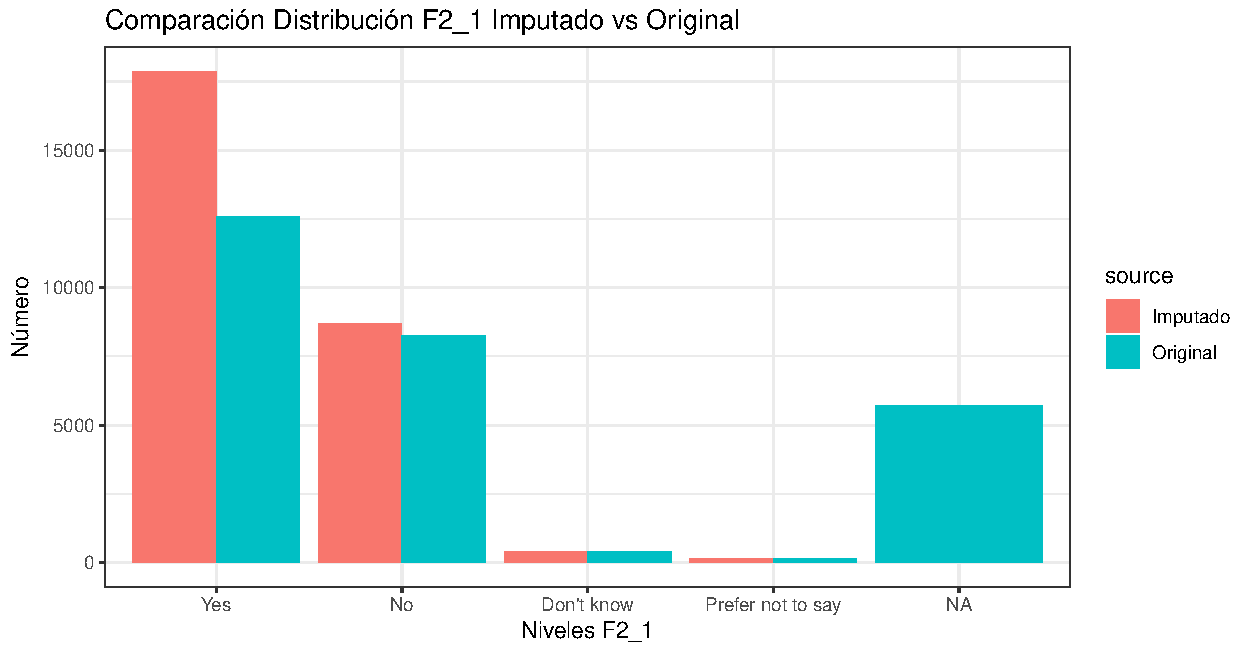
\includegraphics[width=\linewidth]{images/Analysis_MV_F2_1.pdf}
        \caption{Variable F2\_1}
        \label{fig:Analysis_MV_F2_1}
    \end{subfigure}
    \hfill 
    \begin{subfigure}[t]{0.45\linewidth}
        \centering
        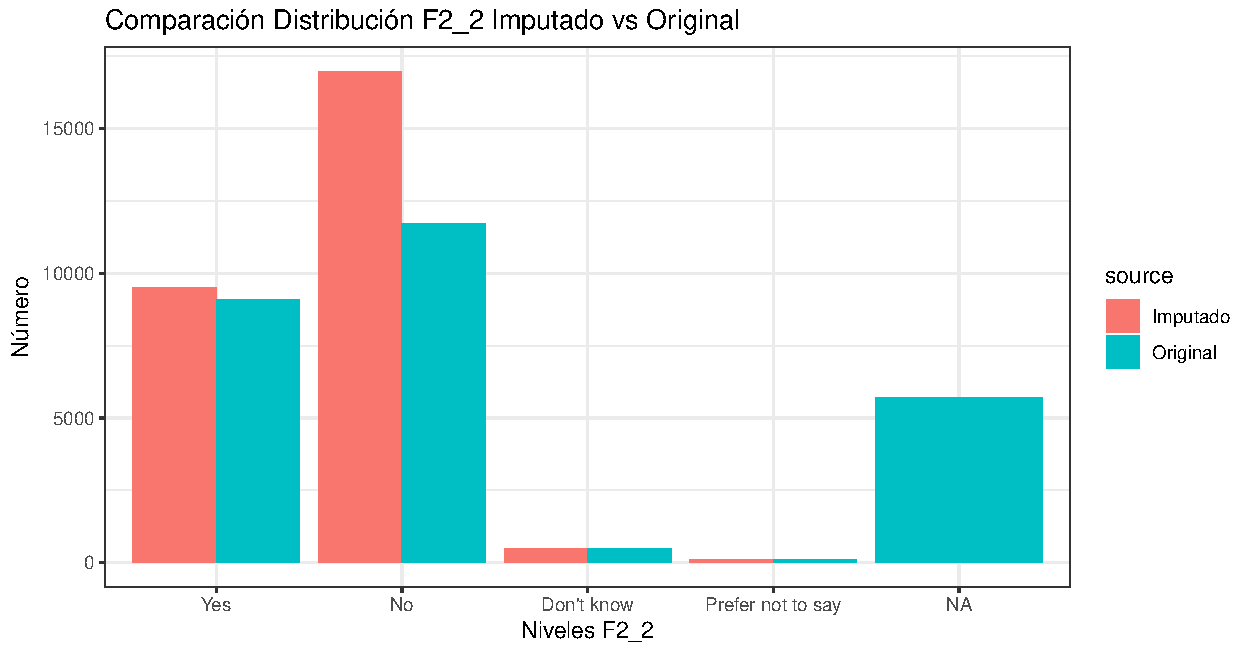
\includegraphics[width=\linewidth]{images/Analysis_MV_F2_2.pdf}
        \caption{Variable F2\_2 }
        \label{fig:Analysis_MV_F2_2}
    \end{subfigure}
    \hfill 
    \begin{subfigure}[t]{0.45\linewidth}
        \centering
        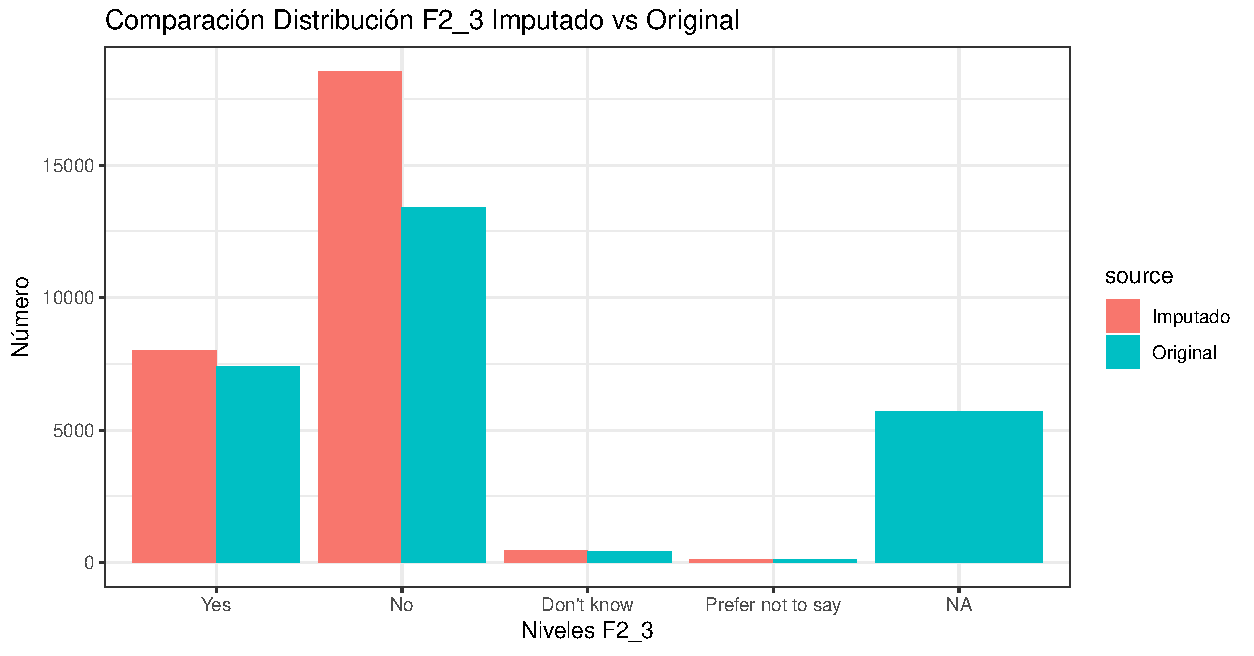
\includegraphics[width=\linewidth]{images/Analysis_MV_F2_3.pdf}
        \caption{Variable F2\_3}
        \label{fig:Analysis_MV_F2_3}
    \end{subfigure}
    \hfill 
    \begin{subfigure}[t]{0.45\linewidth}
        \centering
        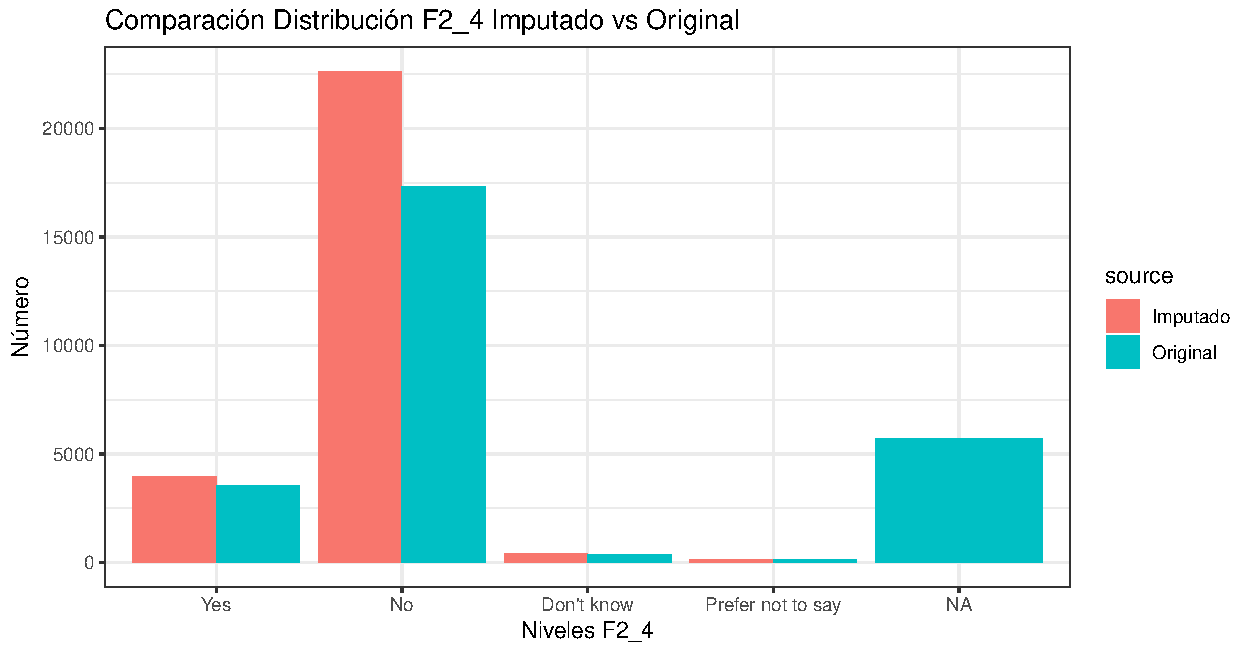
\includegraphics[width=\linewidth]{images/Analysis_MV_F2_4.pdf}
        \caption{Variable F2\_4}
        \label{fig:Analysis_MV_F2_4}
    \end{subfigure}
        \hfill 
    \begin{subfigure}[t]{0.45\linewidth}
        \centering
        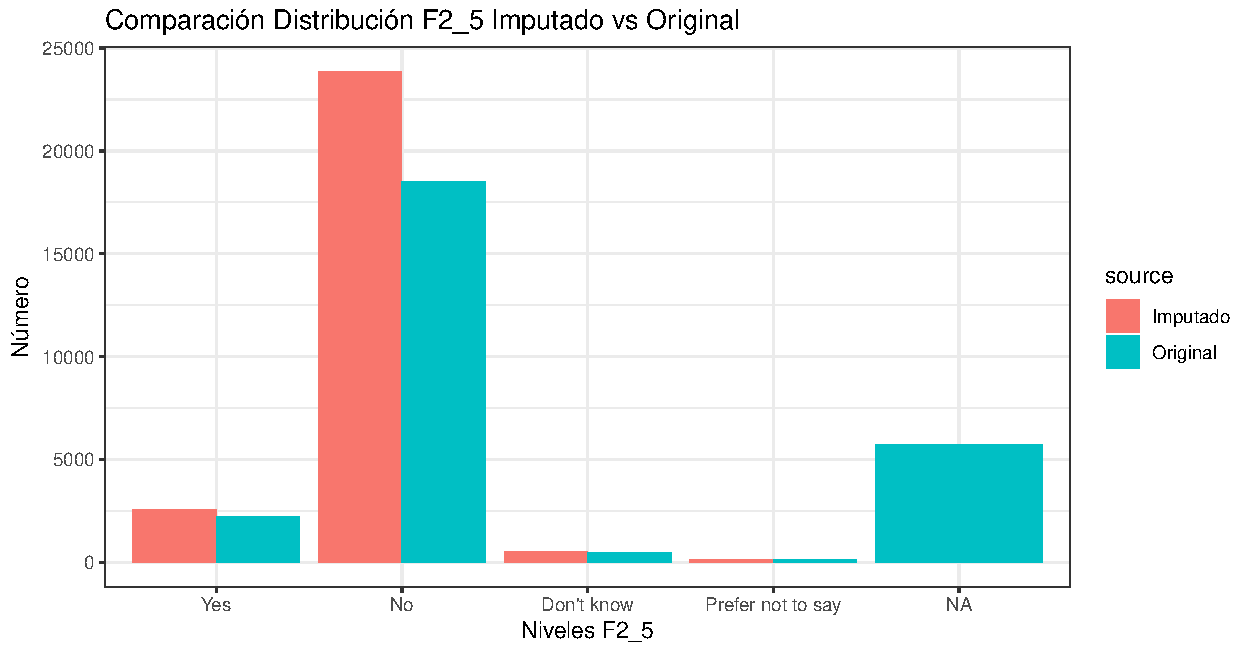
\includegraphics[width=\linewidth]{images/Analysis_MV_F2_5.pdf}
        \caption{Variable F2\_5}
        \label{fig:Analysis_MV_F2_5}
    \end{subfigure}
    \hfill 
    \begin{subfigure}[t]{0.45\linewidth}
        \centering
        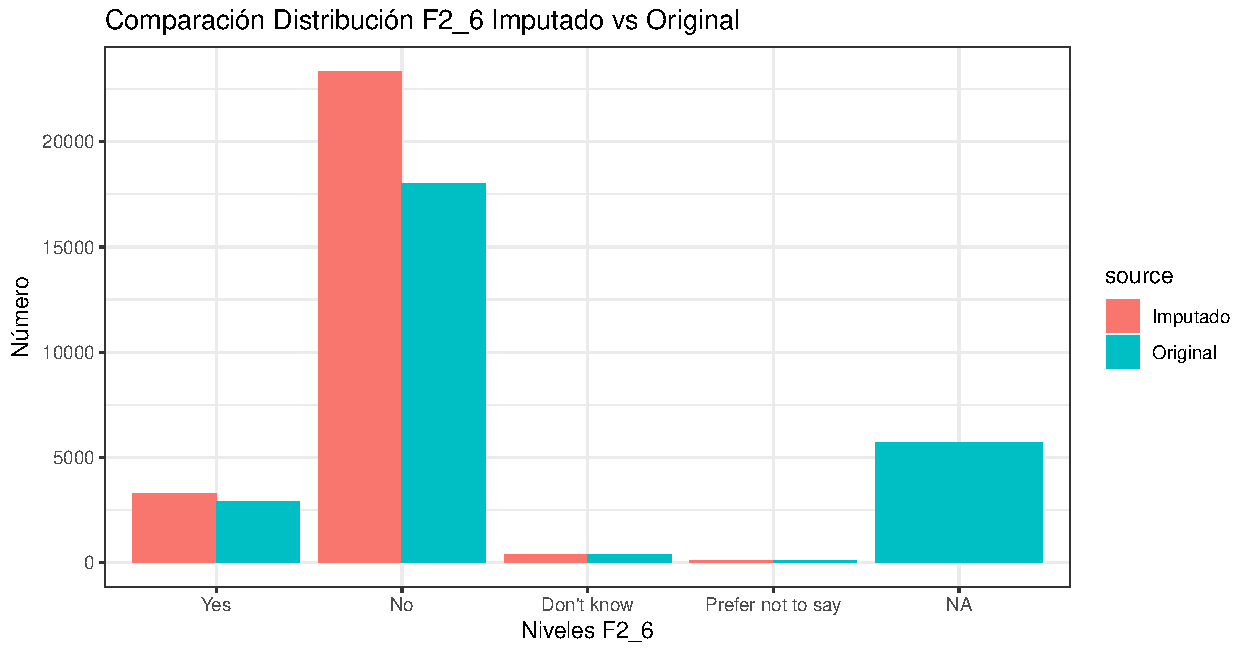
\includegraphics[width=\linewidth]{images/Analysis_MV_F2_6.pdf}
        \caption{Variable F2\_6}
        \label{fig:Analysis_MV_F2_6}
    \end{subfigure}
    \caption{Análisis valores Imputados vs Originales}
    \label{fig:synthetic_analysis}
\end{figure}
\end{center}
\end{document}
